\documentclass[twocolumn]{article}
\usepackage{multicol}
\usepackage[affil-it]{authblk}
\usepackage{amsmath}
\usepackage{tcolorbox}
\usepackage{float}
\makeatletter
\newcommand{\vo}{\vec{o}\@ifnextchar{^}{\,}{}}
\makeatother
\usepackage{graphicx}
\setlength{\parindent}{4mm}
\setlength{\parskip}{0mm}
\renewcommand{\baselinestretch}{1.3}
\begin{document}
%##############################################
%TITLE PAGE
\title{Deterministic Chaos in Classical One Dimensional Scattering}
\author{Andrew Crossman}
\affil{Department of Physics and Astronomy, University of Delaware}
\date{March, 2nd 2019}
\maketitle
\newpage
\twocolumn[
\begin{@twocolumnfalse}
%###############################################
%ABSTRACT
%###############################################
\begin{abstract}
This article will discuss the chaotic behaviors of different sets of initial conditions in a Classical One Dimensional Scattering scenario. The scenario involves a conservative Hamiltonian system that contains two perfectly elastic bouncing balls, which are constrained to an axis that lies parallel to and under the force of Earth's gravitational acceleration. Three main sets of initial conditions will operate on this system and will be analyzed using: $(i)$ Poincar'e Sections constructed by plotting the top ball's position versus its velocity the instance after a collision with the bottom ball; $(ii)$ Positions plots constructed by plotting both balls positions on the axis over time; and $(iii)$ auto-correlation plots constructed by measuring the self-similarity of each ball's positions over time. From these analyses, we will find that the first set of initial conditions is the most chaotic of the three, the second set the most ordered, and the third set a mixture of the two - its top ball being approximately "normal" where as its bottom ball is very chaotic. Aside from these three main sets, we will also construct "modified" sets which we will use to explore the sensitive nature of chaotic systems. The first method we will use to accomplish this is by overlaying modified Poincar'e sections atop one another and observing the drastic structural changes that occur from slight variations in the initial conditions of the system. This sensitivity will be tested by comparing the auto-correlation plots of "modified" sets of initial conditions as well, by showing how small changes can actually cause a chaotic system to become "normal" - or at the very least approximately so. Finally, we will calculate the Lyapunov exponent of a chaotic system and an approximately "normal" system and find that the exponent of the chaotic system is greater than the "normal" one. We reason that this is a sensible conclusion because of the topological mixing that occurs in chaotic systems.  
\end{abstract}
\vspace{5mm}
\end{@twocolumnfalse}
]
%###############################################
%INTRODUCTION
%###############################################
\section{Introduction to Chaos} 
\hspace{\parindent}The study of Deterministic Chaos focuses on the behavior of dynamic systems that are in theory predictable but in practice extremely unpredictable. This stark contrast between the theorists and the experimentalists derives from the properties of chaotic systems as formulated by Chaos Theorist Robert L. Devaney:
\begin{itemize}
  \item sensitivity to initial conditions
  \item topological mixing
  \item dense periodic orbits
\end{itemize}
In general these properties imply that the "exact present determines the exact future," but that the "approximate present does not approximately determine the future." This statement by Devaney directly refers to the predictability of chaotic systems on varying time scales. In relatively short time scales the dynamic features of chaotic systems are actually predictable due to their associative properties of topological mixing and dense periodic orbits. However, given relatively large time scales, these predictions can be thrown completely out the window as the topology of the system will certainly evolve into something else.  

Interestingly enough, the time it takes for the behavior of a chaotic system to evolve can be predicted even if the outcome can not be. This determination depends on two things: the accuracy at which the current state can be measured and a time scale called the Lyapunov time which depends on the dynamics of the system. With greater accuracy in measurements, comes a smaller uncertainty in the time frame of the next topological change, and with a greater Lyapunov time, comes a larger period of time before next topological change. These characterizations and properties of chaotic systems are very important to understand because they help us explain many natural phenomena such as weather and climate, which are essentially billions and billions of atoms all interacting with each other. Chaotic systems can also arise spontaneously in some systems with artificial components, such as with pedestrian traffic in large cities and popular support for government policies. 

The goal of this particular experiment, is to explore the behavior of a chaotic system that is much simpler than climate or traffic, in order to gain a fundamental understanding and intuition about chaotic systems that would not be possible when many many degrees of freedom are present. Hence, this experiment will revolve around the two degrees of freedom present in a conservative Hamiltonian system that contains two infinitesimally small balls constrained to, and moving along, an axis that is parallel to the force of gravity. The balls' collisions between each other and with the floor will be perfectly elastic and will not deform the balls in any way. The lower of the two balls will be denoted as ball one, and the higher of the two as ball two. They will have respective masses, positions, and velocities $m_1$, $m_2$, $x_1$, $x_2$, $v_1$, $v_2$ and will only be acted upon by the Earth's force of gravity.
%###############################################
%Methodology
%###############################################
\section{Methodology}
\hspace{\parindent} 
In order to properly observe and analyze our Hamiltonian system it will be evaluated using an analytic approach. Using the "pen and paper" method we will first, normalize the Kinematic Equations of Motions that describe the positions and velocities of the two balls over time. Then, we will virtually construct the simulation and apply our normalized Kinematic Equations to the balls for the duration of time that it takes one thousand collisions to occur for each of the three sets of initial conditions. During the time it takes these one thousand collisions to occur we will record the $x_2$ and $v_2$ values at the instance after the two balls collide. Next, we will take this time duration and subdivided into one million time steps of equal size. Using these steps, we will run the simulation again, but instead of recording $x_2$ and $v_1$ after each collision we will record $x_1$, $v_1$, $x_2$, and $v_2$ at each time step. It is imperative throughout this process that particular attention is payed to whether or not a collision or floor bounce occurred in the period of time between steps. If one of these events did occur - which would be indicative of their positions being in impossible ranges due to the constraints $x_1<x_2$ and $x_1>0$ - then the updated quantities must be corrected to ensure accurate simulation results. After the quantities are all accounted for, for each time step, we will find the auto-correlation of the positions of both $x_1$ and $x_2$ by applying the formula:
$$C(\tau)=\int_{0}^{\infty}[x(t)-\bar{x}][x(t+\tau)-\bar{x}]dt$$
to the first $50^{th}$ of their positions compared to the rest of their respective positions over time (this time length was chosen so that the calculations would not take unreasonably long). At this point - now that we have all the necessary data - we will construct Poincar'e plots by plotting $x_2$ versus $v_2$, Position plots by plotting $x_1$ and $x_2$ versus time, and Auto-Correlation plots by plotting $x_1-autocorrelation$ and $x_2-autocorrelation$ versus a subsection of time for each set of our initial conditions. Having constructed our data sets into a more digestible form, we will then compare our plots against each other and comment on the differences and similarities that evolved from their chaotic systems. Finally, we will study and explore the respective Lyapunov exponents for both the chaotic and non-chaotic case of $m_2=9m_1$ when their initial $x_2$ positions are increased by $10^{-6}$ at the start.
\section{Normalization}
\hspace{\parindent} The Kinematic Equations of Motion are a set of equations that can be used to predict an object's motion if certain information - such as the object's velocity and position - is known. The equations only work when when an object experiences either a constant velocity or a constant acceleration, which conveniently for us happens to be exactly the case of our system, since it is only affected by a gravitational field with magnitude $g$. Hence, these equations will work for our purpose of accurately calculating the positions and velocities of our system's balls. Typically these equations are written in the form:
\begin{align}
	x_{final} &= x_i + vt + \frac{at^{2}}{2} \\
	v_{final} &= v_i + at \\
	v_{final}^{2} &= v_i^{2} + 2a\delta x
\end{align}
In our case however, we want to normalize these equations with scaling constants that are constructed from fundamental constants of the system. These fundamental constants can be things such as the constant energy of the conservative system, the constant acceleration of gravity, or the constant mass. The goal of doing this is to hopefully observe some fundamental structures of the system that would not be discernible otherwise. Keeping this in mind then, these scaling constants are:
\begin{align}
	x_o = \frac{E}{mg} \\
	v_o = \sqrt{\frac{E}{m}} \\
	t_o = \sqrt{\frac{E}{mg^{2}}}
\end{align}
where $E$ is the total energy of the system, $m$ is the total mass of the system, and $g$ is the force of gravity. Now that we have our scaling constants - with appropriate units - we can scale the components of the system that are relevant to their Kinematic Equations. Hence we find that our Normalized quantities are...
\begin{align}
	\grave{x} &= \frac{x}{x_o} \\
	\grave{v} &= \frac{v}{v_o} \\
	\grave{t} &= \frac{t}{t_o}
\end{align}
where $\grave{x}$ $\grave{v}$, and $\grave{t}$ are our correctly scaled units. If we substitute these units into our Kinematic Equations we also find that equation $(1)$ becomes...
\begin{align}
	\grave{x}_fx_o &= \grave{x}_ix_o + \grave{v}v_o\grave{t}t_o - \frac{g\grave{t}^{2}t_o^{2}}{2} \\
	\grave{x}_f\frac{E}{mg} &= \grave{x}_i\frac{E}{mg} + \sqrt{\frac{E}{mg^{2}}}\sqrt{\frac{E}{m}}\grave{v}\grave{t} - \frac{g\grave{t}^{2}E}{2mg^{2}} \\
	\grave{x}_f &= \grave{x}_i + \grave{v}\grave{t} - \frac{\grave{t}^{2}}{2}
\end{align}
Equation $(2)$ becomes...
\begin{align}
	\grave{v}_fv_o &= \grave{v}_iv_o - g\grave{t}t_o \\
	\grave{v}_f\sqrt{\frac{E}{m}} &= \grave{v}_i\sqrt{\frac{E}{m}} - g\grave{t}\sqrt{\frac{E}{mg^{2}}} \\
	\grave{v}_f &= \grave{v}_i - \grave{t}
\end{align}
And Equation $(3)$ becomes...
\begin{align}	
	\grave{v}_f^{2}v_o^{2} &= \grave{v}_i^{2}v_o^{2} - 2g\delta\grave{x}x_o \\
	\grave{v}_f^{2}\frac{E}{m} &= \grave{v}_i^{2}\frac{E}{m} - \frac{2gE}{mg}\delta\grave{x} \\
	\grave{v}_f^{2} &= \grave{v}_i - 2\delta\grave{x}
\end{align} 
where, our Normalized Kinematic Equations of Motion are equations $(12)$, $(15)$, and $(18)$. 

We should note at this time that the normalized unit of $g$ is merely $\grave{g}=1$. This is because the scaling factor of $g$, when constructed in fundamental constants of the system, is itself. Hence, $g_o=g$, and therefore $\grave{g}=\frac{g}{g_o}=1$. This is important to realize, despite its complete cancellation with-in the Kinematic Equations because it is still present in the Normalized Energy Equation:
\begin{align}
\grave{E}=1=\frac{m_1}{2m_2}\grave{v}_1^{2}+\frac{m_2}{2m}\grave{v}_2^{2}+\frac{m_1}{m}\grave{g}\grave{x}_1+\frac{m_2}{m}\grave{g}\grave{x}_2
\end{align}
Also note that $\grave{E}$ is equal to one in this normalization because we are constraining all of our systems to the same energy.
\section{Energy and Collisions}
\hspace{\parindent} Aside from our Normalized Kinematic and Energy equations, we still need to calculate the quantities necessary to construct our scaling factors as well as to determine the velocities of the balls after their collisions. Given that our system is conservative, we know that the total energy of the system is constant and can be calculated by the Kinetic-Work Energy Theorem. In the case of our system this takes the form:
\begin{align}
	E = \frac{1}{2}m_1v_1^{2} + \frac{1}{2}m_2v_2^{2} + m_1gx_1 + m_2gx_2
\end{align}
where the variables are the previously discussed properties of ball one and ball two and $E$ is the required quantity need for our scaling factors. The total mass of the system is much more simple to calculate:
\begin{align}
	m = m_1 + m_2
\end{align}
where $m$ is another of the required quantities needed for our scaling factors. The final quantity $g$, is just the magnitude of the gravitational field of Earth which is $9.807 \frac{m}{s^{2}}$.

Having acquired all we need for our scaling factors and Normalizations, let us discuss the consequences of the balls collisions with each other and the floor. In the case that ball one hits the floor its velocity vector will reverse due to its perfect elasticity property. In the case of ball two, it will never collide with the floor because its lower height bound is constrained by the height of ball one, which is always below it. In the case that the balls collide with one another, the balls' velocities will change in accordance to the rules of perfect elasticity which entail a conservation of momentum and a conservation of kinetic energy. That is to say that the collisions will abide by the equations:
\begin{align}
	m_1v_{1i} + m_2v_{2i} &= m_1v_{1f} + m_2v_{2f} \\
	m_1v_{1i}^{2} + m_2v_{2i}^2 &= m_1v_{1f}^{2} + m_2v_{2f}^{2}
\end{align}
Rearranging these equations and solving for the balls' velocities we find that...
\begin{align}
	v_{1f} &= \frac{m_1-m_2}{m_1+m_2}v_{1i} +\frac{2m_2}{m_1+m_2}v_{2i} \\
	v_{2f} &= \frac{2m_1}{m_1+m_2}v_{1i} + \frac{m_2-m_1}{m_1+m_2}v_{2i}
\end{align}
where $v_{1f}$ and $v_{2f}$ are the velocities of the balls the instance after their collision. Note we do not need to manually reverse either of their velocities as in the case of ball one hitting the floor because these equations account for the velocity vector.
\section{Analysis}
\hspace{\parindent}Now that we gone through and explained the processes through which we have created our simulation, it is time that we organize and examine the produced data in a meaningful form. We will accomplish this by first, creating Poincar'e Sections based off of several sets of initial conditions and observing their general structures and substructures. Then we will explore the position plots of the same several sets of initial conditions and distinguish particular "dense periodic orbits." Following that we will examine the auto-correlation functions of each set and comment on the "amount" of chaos present in the different systems. Finally, we will observe how very small changes in the initial conditions of a system can cause dramatically different outcomes over time by computing the Lyapunov exponent for both a chaotic and "normal" set of initial conditions.
\subsection{Poincar'e Sections}
\hspace{\parindent}Poincar'e sections otherwise known as first recurrence maps, allow us to discern patterns of motion within large complex structures that are seamlessly random. They preserve many of the properties of the quasi-periodic orbits of the overall system, and are conveniently plotted as a function of space rather than time. For our specific plots we will look at the normalized space composed of $x_2$ versus $v_2$. Plotting our three sets of initial conditions we find: \\
\begin{figure}[h]
\caption{$m_1=1$, $m_2=0.5$, $x_1=1$, $x_2=3$, $v_1=0$, $v_2=0$}
\centering
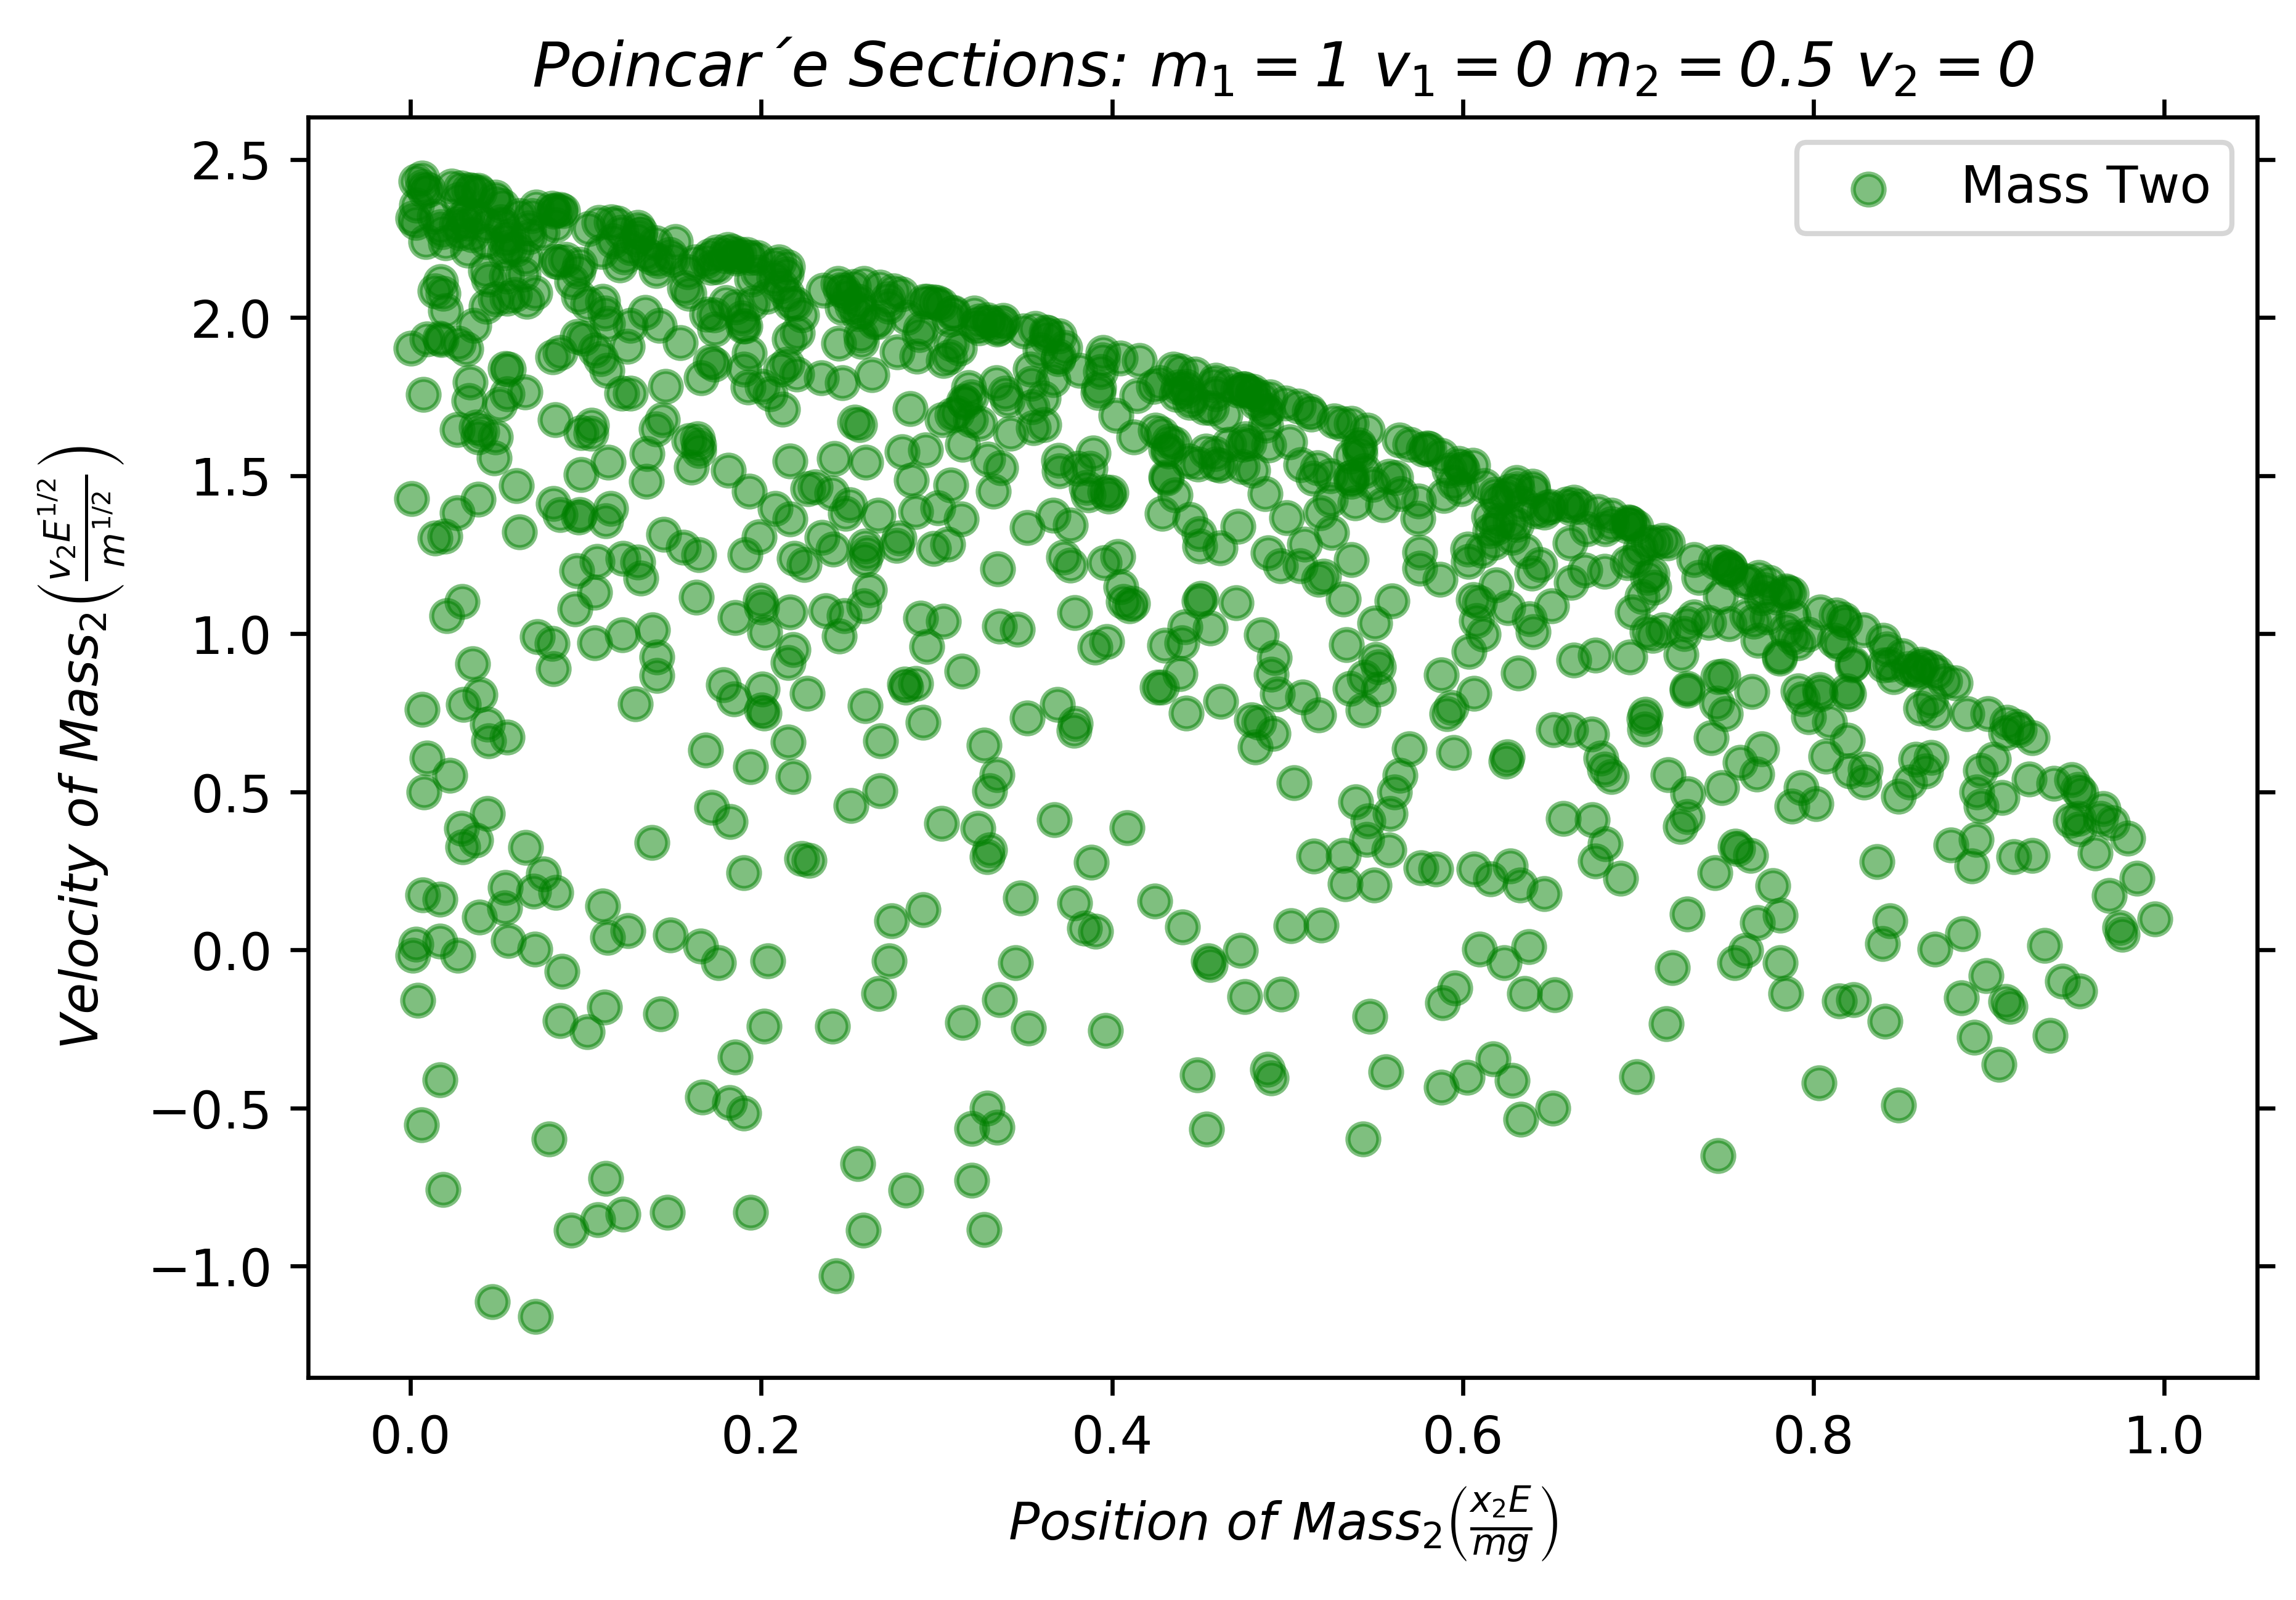
\includegraphics[scale=.45]{Section-IC1-Scatter}
\end{figure} 
\begin{figure}[h]
\caption{$m_1=1$, $m_2=1$, $x_1=1$, $x_2=3$, $v_1=0$, $v_2=0$}
\centering
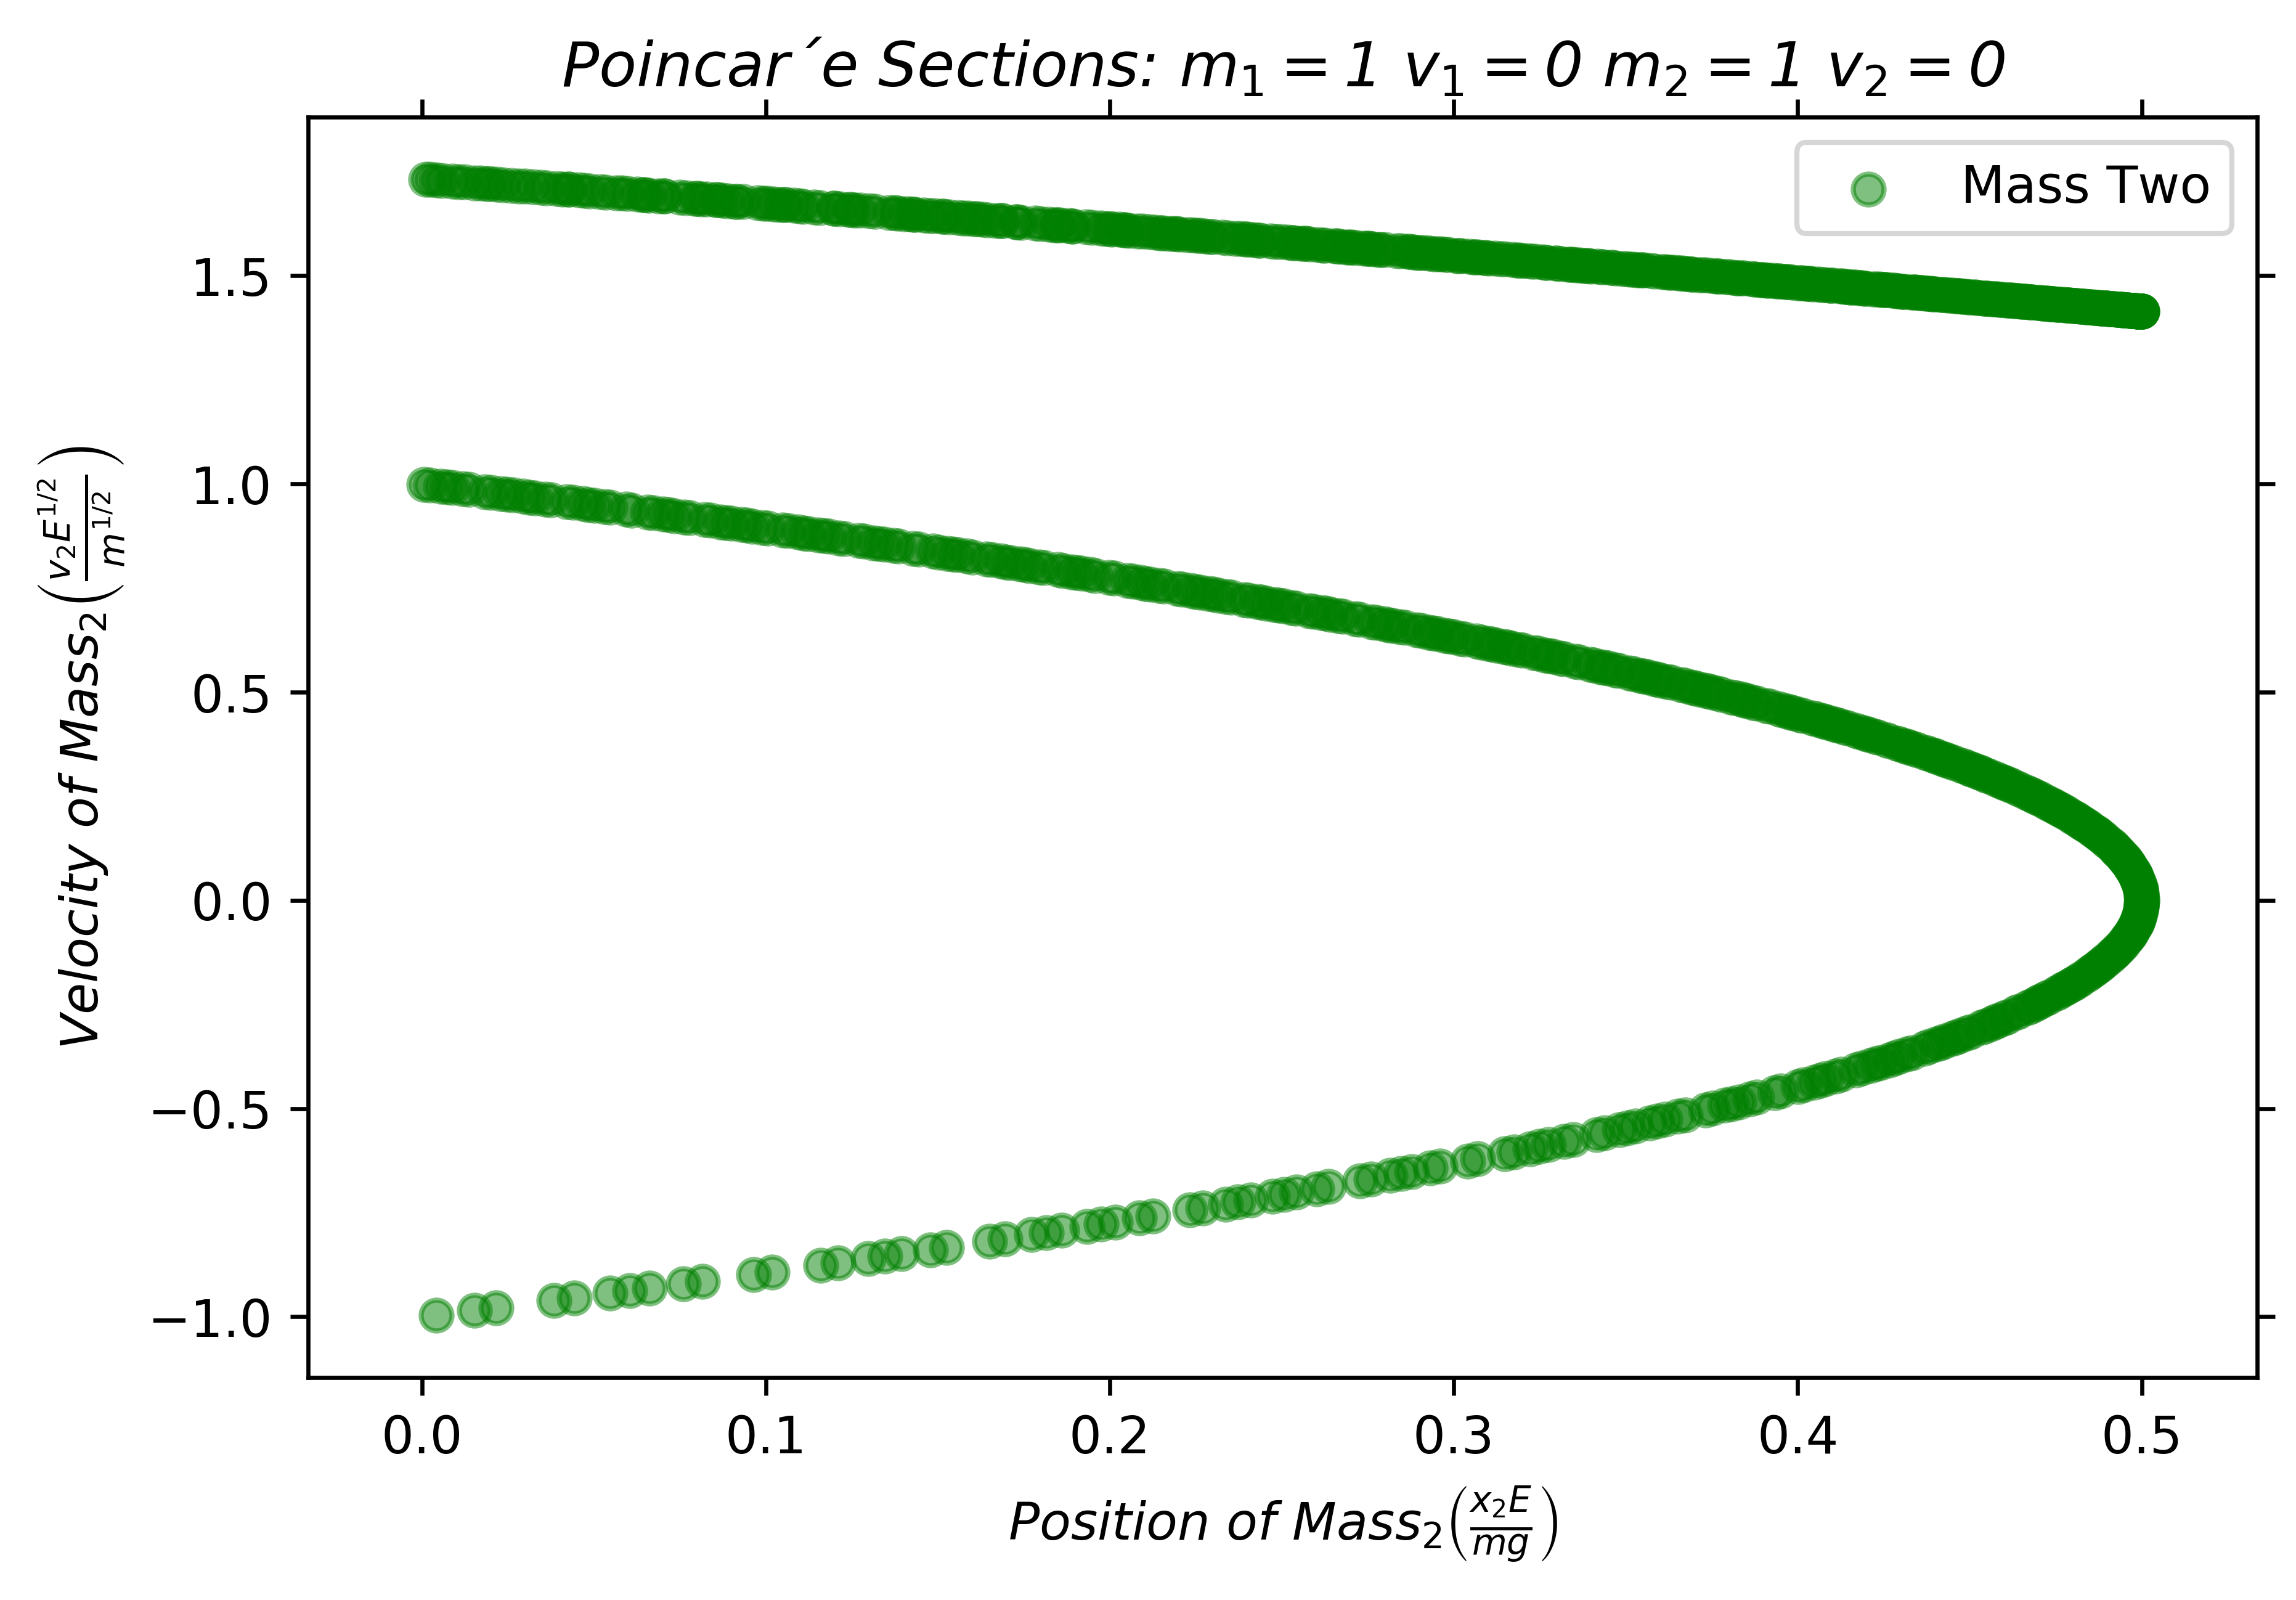
\includegraphics[scale=.45]{Section-IC2-Scatter}
\end{figure}
\begin{figure}[h]
\caption{$m_1=1$, $m_2=9$, $x_1=1$, $x_2=3$, $v_1=0$, $v_2=0$}
\centering
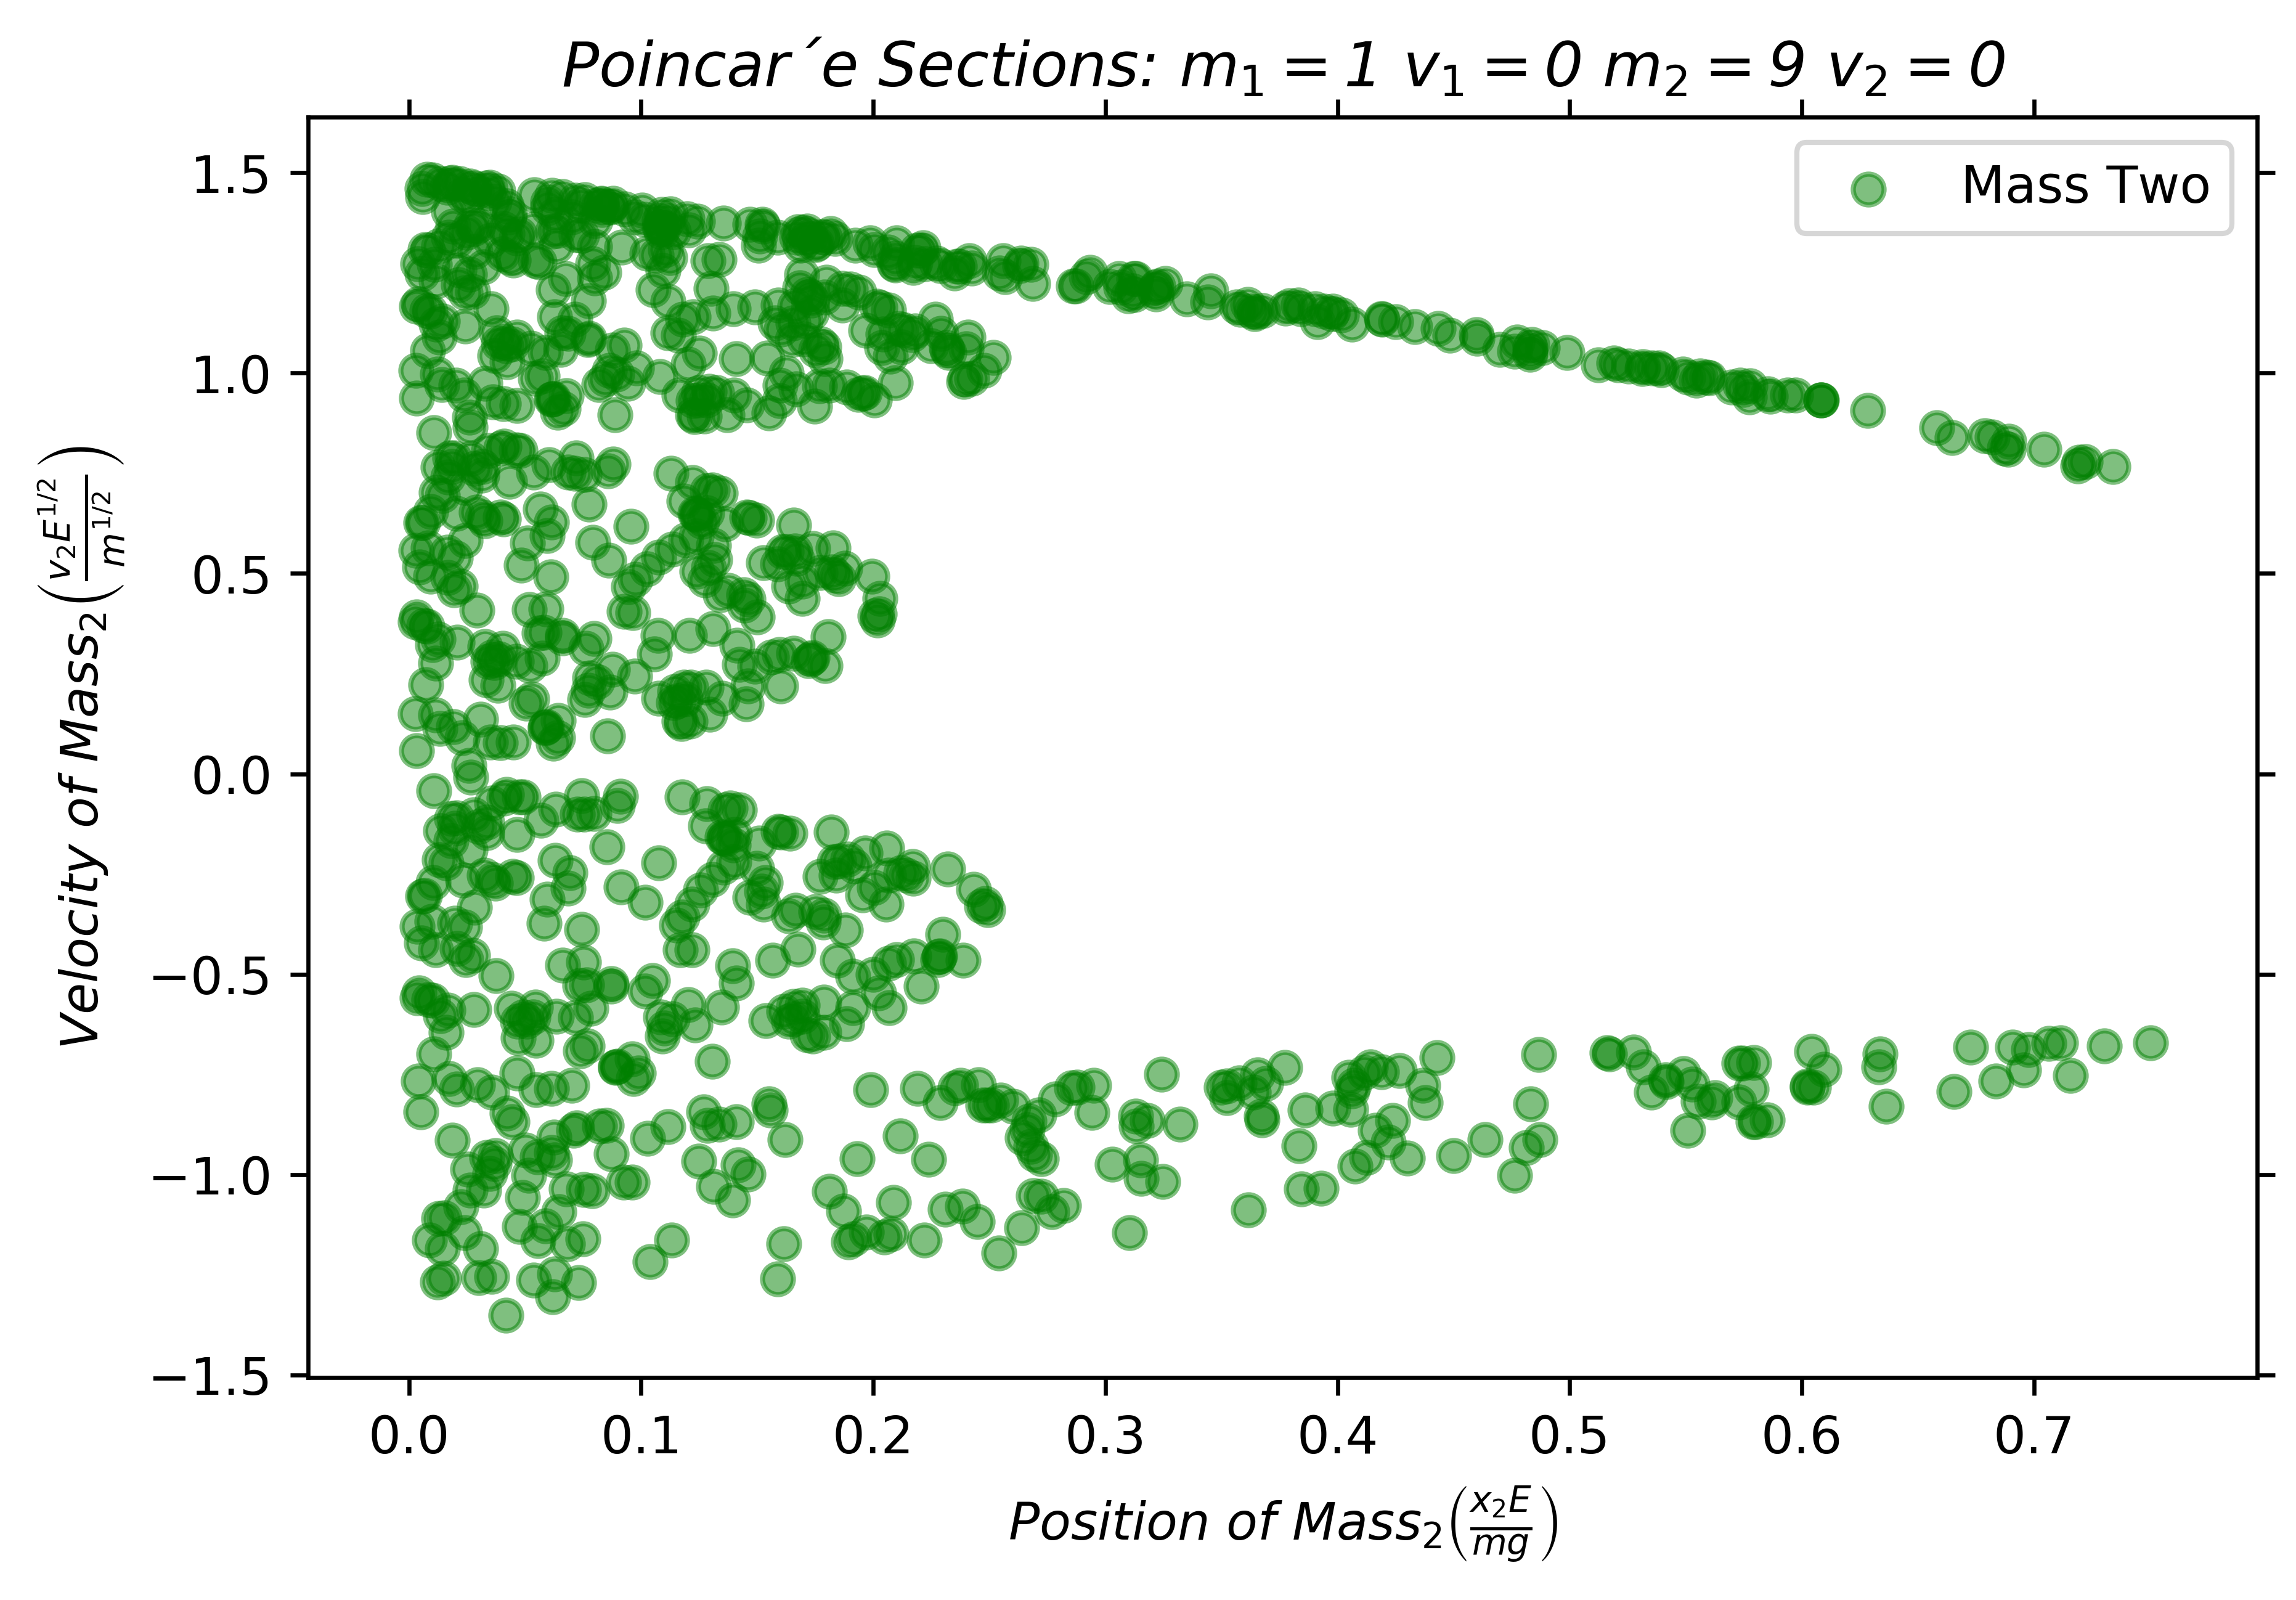
\includegraphics[scale=.45]{Section-IC3-Scatter}
\end{figure}
\hspace{-3.8mm}Clearly, there exists distinct structural differences between the three sets of initial conditions. The first set (Figure 1) appears to be very scattered and disorder, and only has one real area that can even begin to be called a structure - this being the denser region that runs along the upper edge of the figure. The second set (Figure 2) unarguably, has two very "clean," ordered, and distinct structures, which is a sharp contrast to set one's features. The third set (Figure 3) on the other hand, appears to have qualities of both the former sets. There certainly exists distinguishable structures with-in its figure unlike set one's; however, these structures are certainly not as ordered and "clean" as in set two's case. In terms of how "chaotic" each set of conditions are then, it is probably safe to say that the first set is the most chaotic as it is the most random, the second set the least as it is the most ordered, and the third set the second most as it is neither the most random nor the most ordered.

Now that we have an understanding as to how to interpret these plots, lets look at exactly how sensitive these systems are in regards to their initial conditions. We will do this by taking the second set's (Figure 2) initial conditions and make small adjustments to them twelve times. We will then construct Poincar'e sections for each of these modified sets and overlay them on top of one another to view them all at once. Recall that the initial conditions for the second set are $m_1=1$, $m_2=1$, $x_1=1$, $x_2=3$, $v_1=0$, $v_2=0$, where as our twelve new sets will either change the positions and velocities by no more than one, or change the masses to $m_1=1.01$ and $m_2=.99$, $m_1=1$ and $m_2=3$, $m_1=1$ and $m_2=4$, or $m_1=1$ and $m_2=5$. Hence, we find...
\begin{figure}[H]
\caption{Overlapping Conditions}
\centering
\includegraphics[scale=.5]{Section-MultiConditions1}
\end{figure}
\hspace{-3.8mm}where each color represents a different set of initial conditions (see $project2$\textunderscore$crossman.py$ function multipoincare() for more details on the ICs). Evidently, the slight changes we made to the original initial conditions of Figure 2 created dramatically different structures. By testing the parameters individually, you can find that the greatest structural changes came from altering the masses rather than the initial positions or velocities. Changes in mass - even at the $.01$ scale - caused the entire structure of the Poincar'e Section to change, where as alterations to the initial positions and velocities for the most part just resulted in the same structures as Figure 2 but elongated or truncated along the axes. Hence, even minute differences between the initial starting conditions can cause drastic changes in the topology of the system.
\subsection{Position Plots}
\hspace{\parindent} Now that we have explored the spacial aspects of our different initial sets, lets investigate their time dependencies. Before we take a look at the actual data however, it is always good to test our intuition about the problem based on prior knowledge (i.e. our Poincar'e Sections). We know that set one was very chaotic and so in theory we should expect the balls' positions versus time to appear similarly randomly. In the case of set two, we know that there were two clearly defined structures. Hence, its positions versus velocities should be similarly distinct or periodic. In the case of set three, we know that there were distinguishable structures but that they were not as distinct or ordered as in the second set. Hence, we should expect some periodic evolutions to  occur. \\
\begin{figure}[H]
\caption{$m_1=1$, $m_2=0.5$, $x_1=1$, $x_2=3$, $v_1=0$, $v_2=0$}
\centering
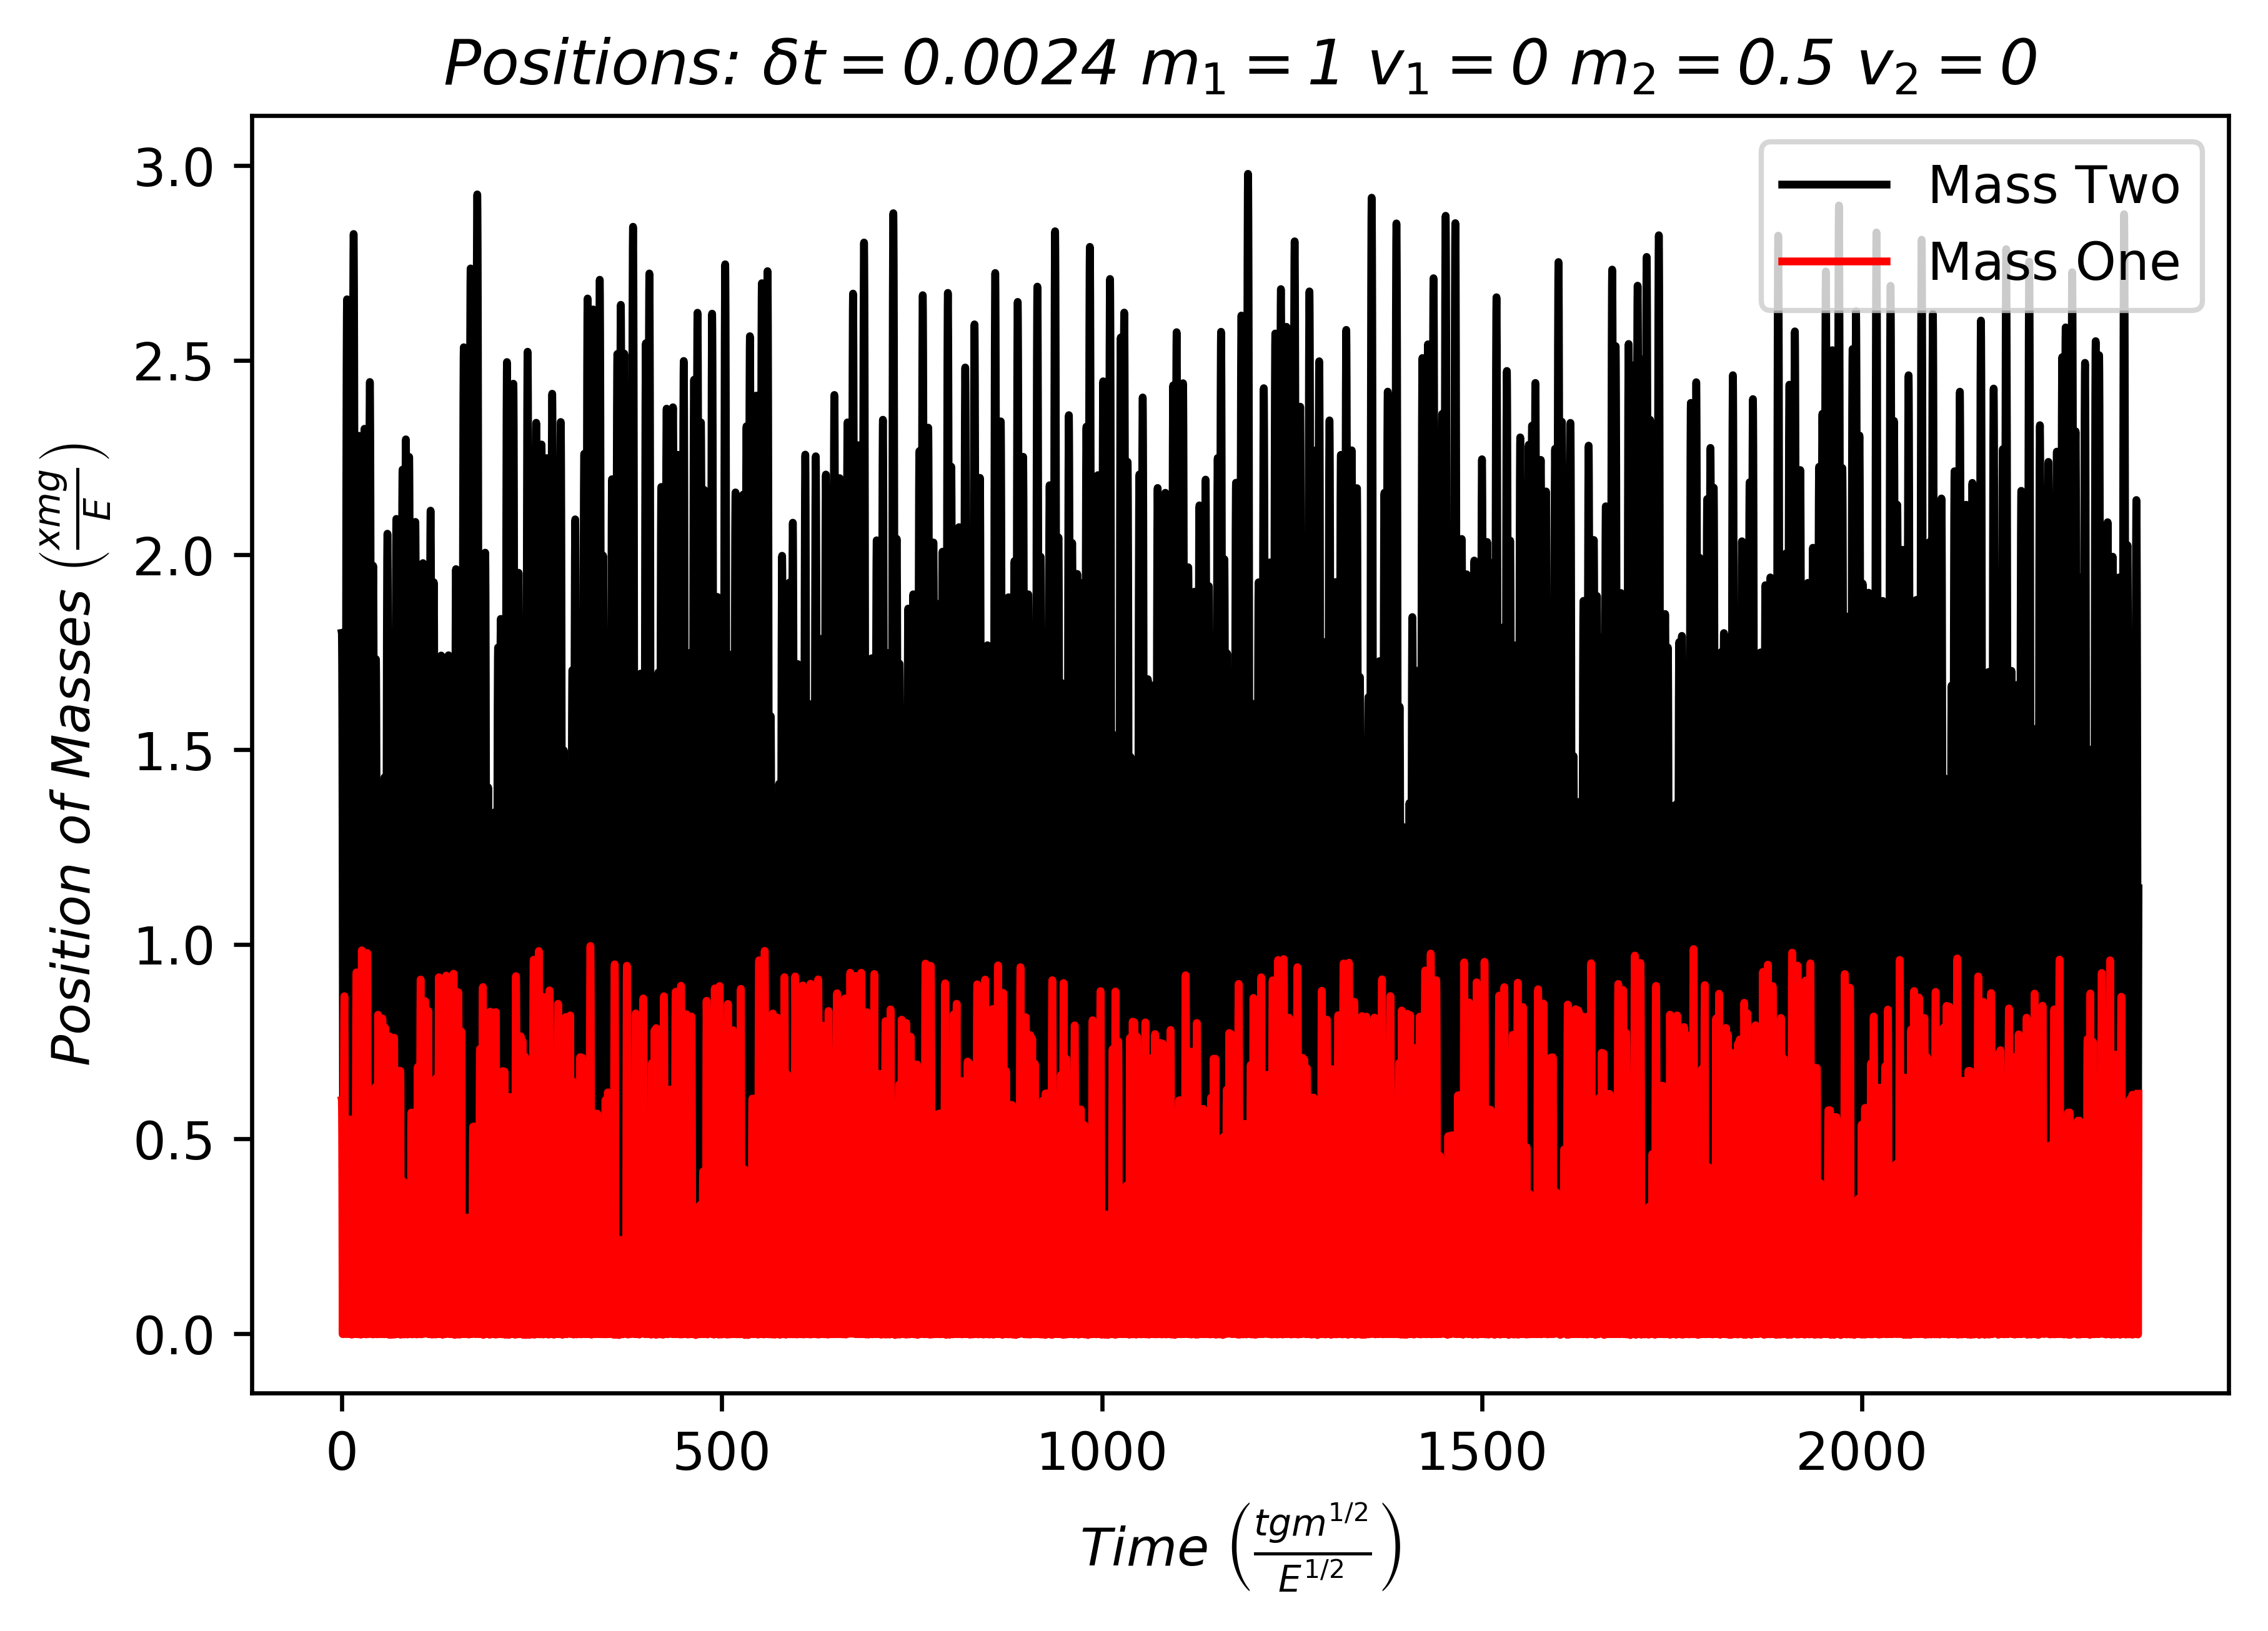
\includegraphics[scale=.45]{Positions-MassOne1MassTwo0-5x1i1x2i3}
\end{figure}
\begin{figure}[H]
\caption{$m_1=1$, $m_2=1$, $x_1=1$, $x_2=3$, $v_1=0$, $v_2=0$}
\centering
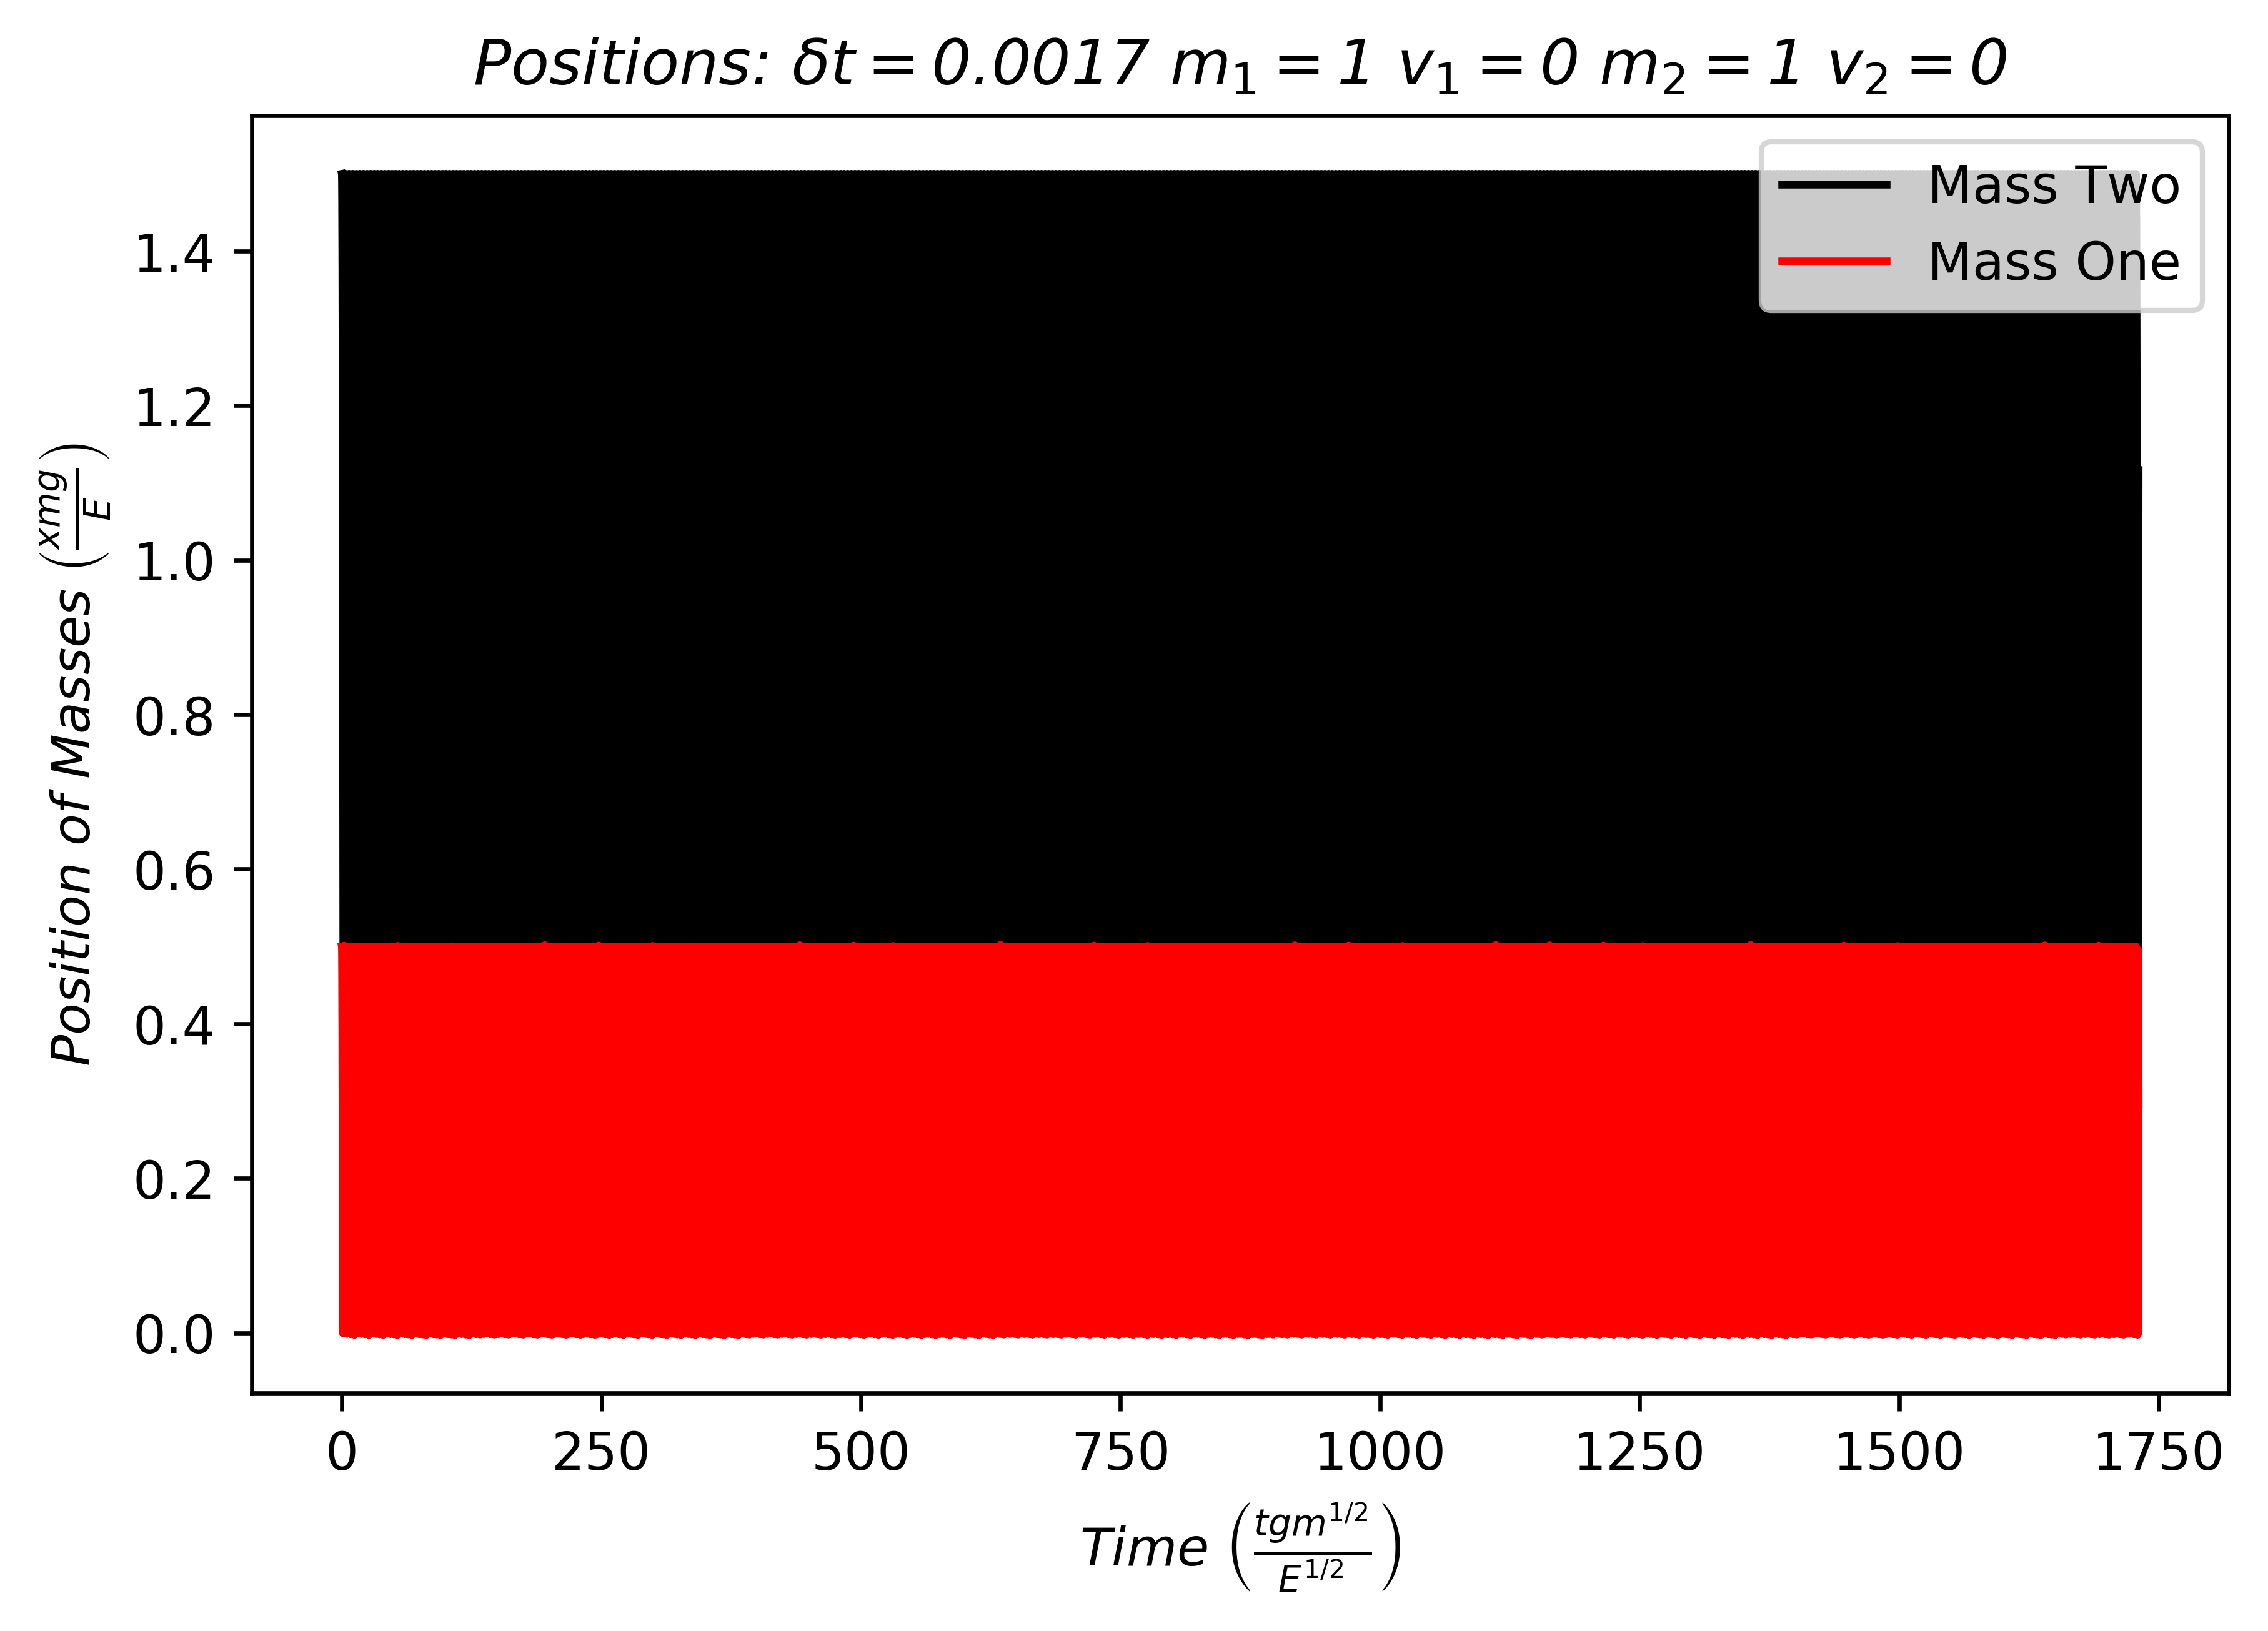
\includegraphics[scale=.45]{Positions-MassOne1MassTwo1x1i1x2i3}
%\end{figure}
%\begin{figure}[h]
\caption{$m_1=1$, $m_2=9$, $x_1=1$, $x_2=3$, $v_1=0$, $v_2=0$}
\centering
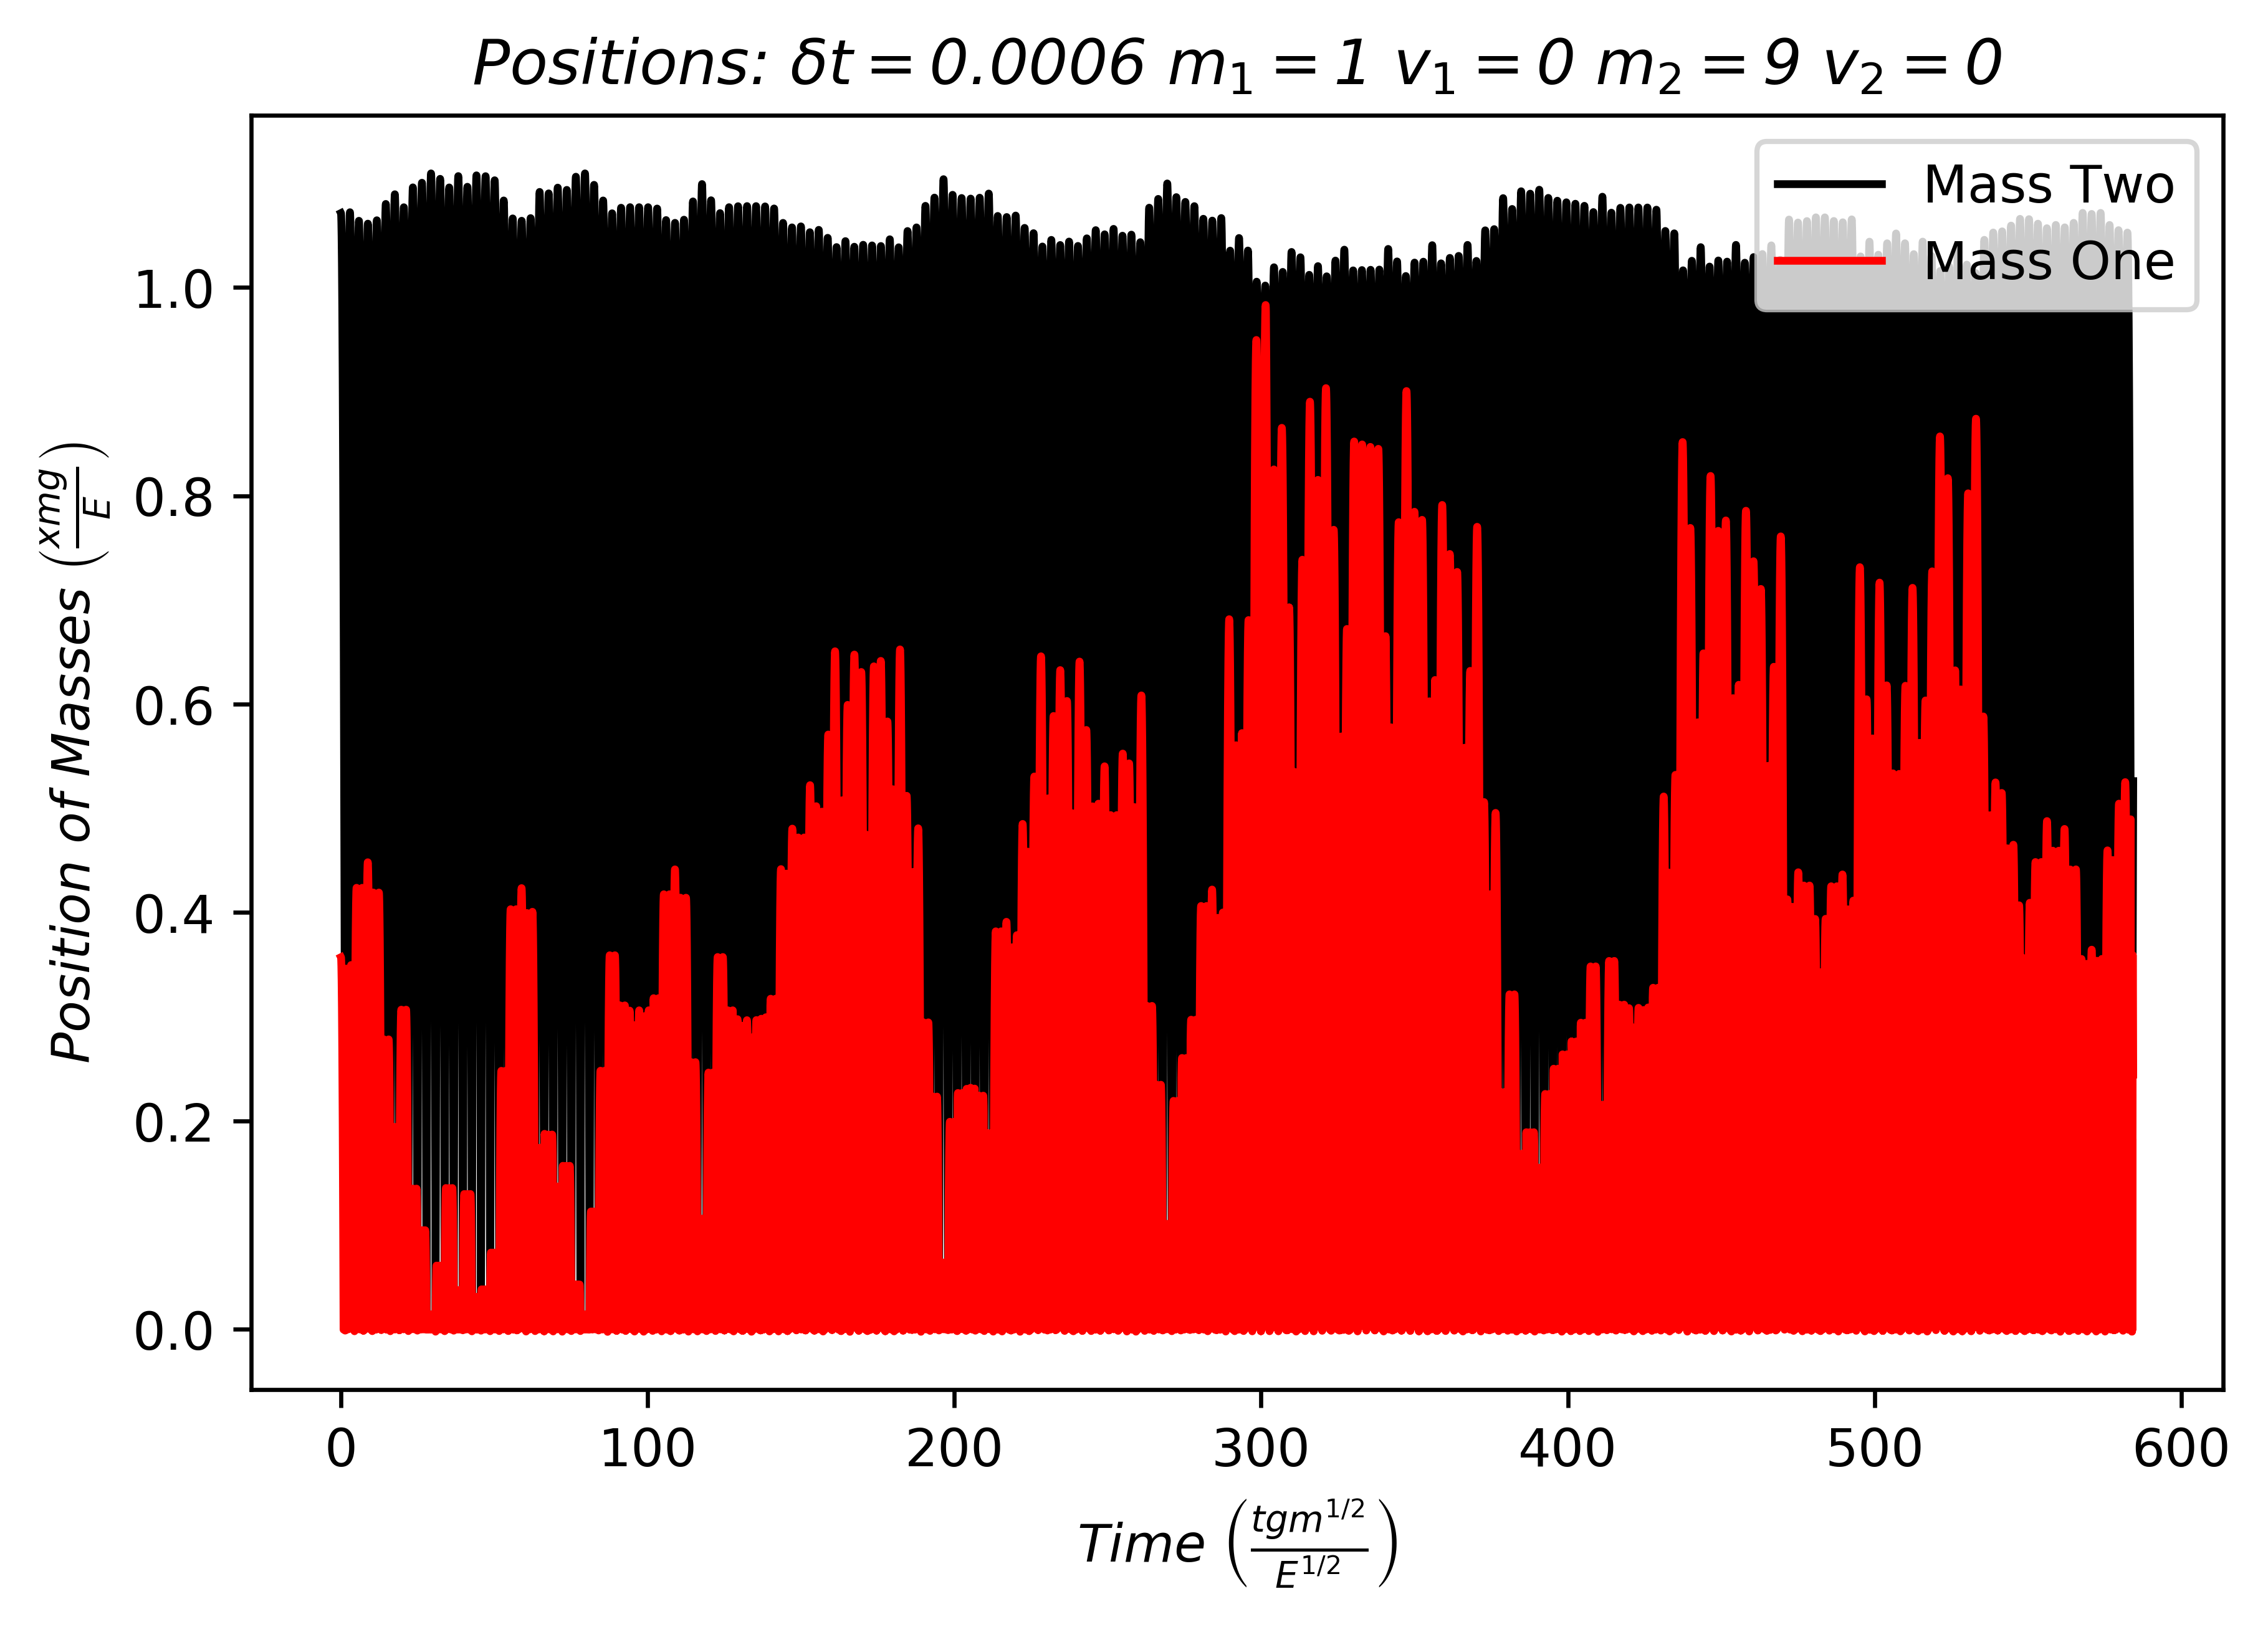
\includegraphics[scale=.45]{Positions-MassOne1MassTwo9x1i1x2i3}
\end{figure}
Looking at our plots, it would appear that predictions were correct! Set one's plot (Figure 5) does indeed appear to be quite disordered and random. Set two's plot (Figure 6) on the other hand is very consistent and ordered - to the point that it looks like to thick lines. Set three's plot (Figure 7) is also characterized by numerous periodic changes as we expected, though it should be noted as a point of interest that there are more periodic changes here than there were structures within the Poincar'e section. If we zoom in on these plots we can also ensure the accuracy of our model by visually confirming that the balls collide correctly with the floor and each other. We can use these zoomed plots to discern the periodic structures at the period of time that the zoom extends for as well. \\
\begin{figure}[h]
\caption{$m_1=1$, $m_2=0.5$, $x_1=1$, $x_2=3$, $v_1=0$, $v_2=0$}
\centering
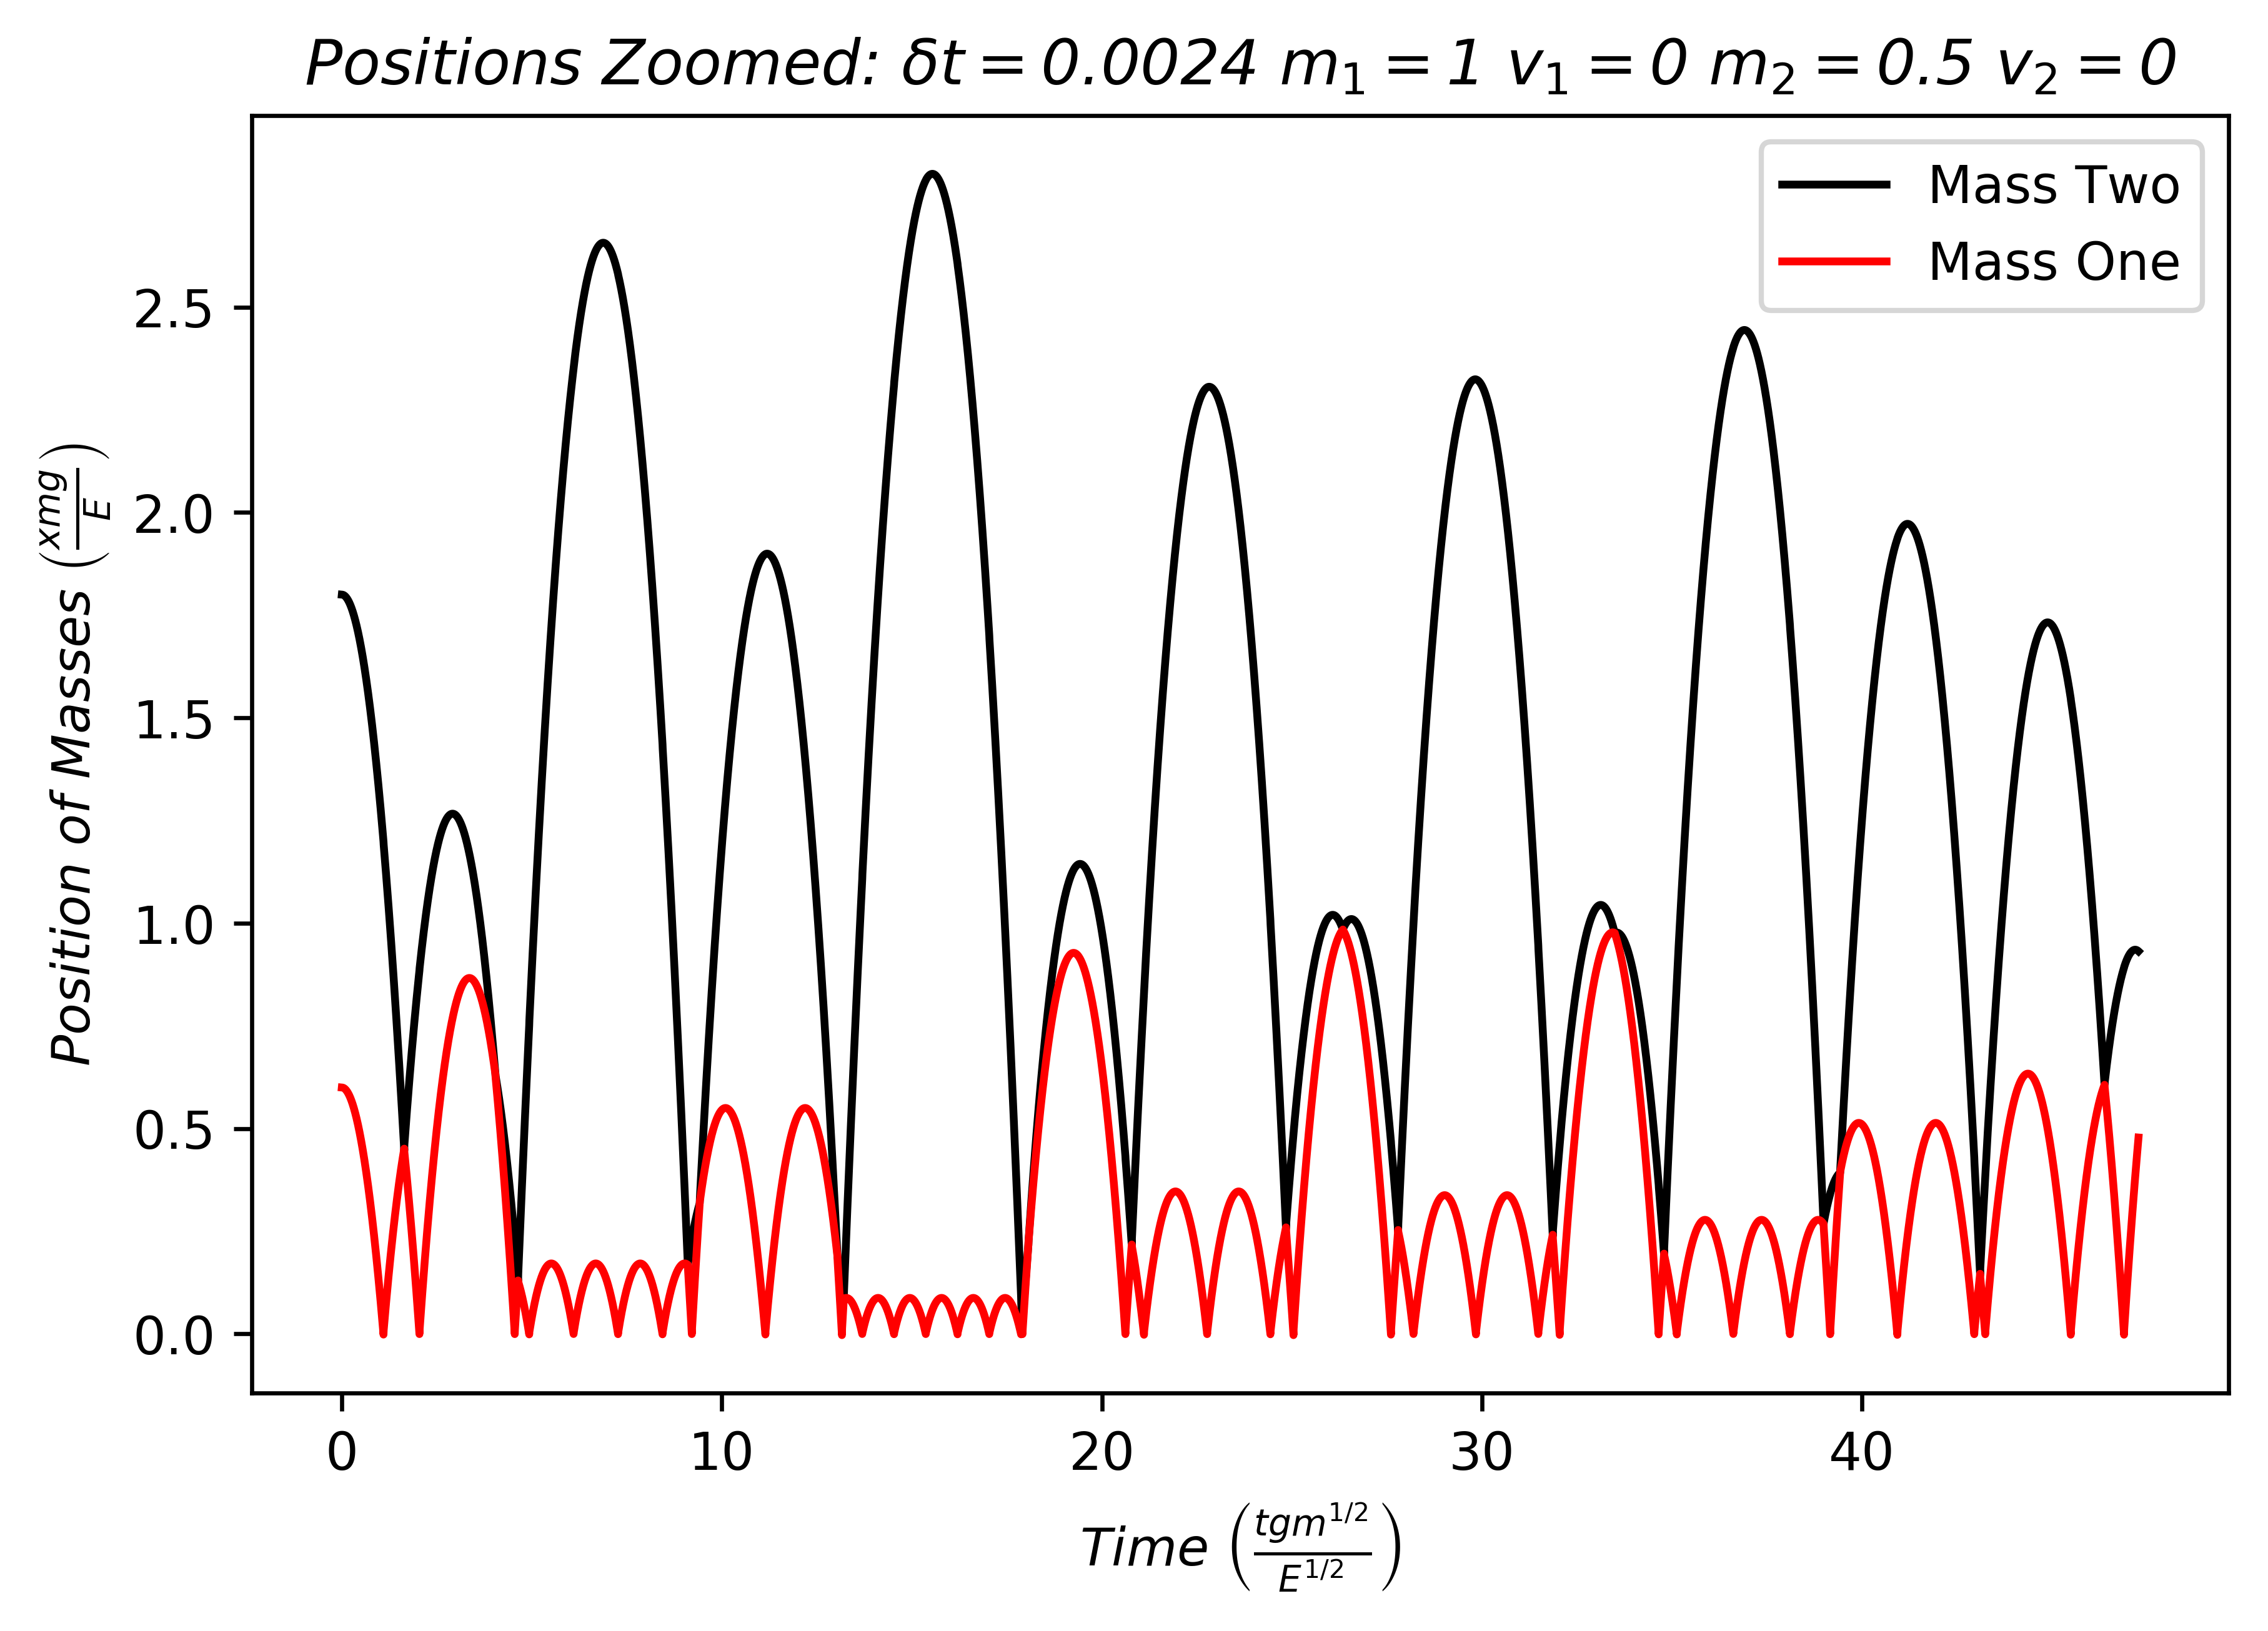
\includegraphics[scale=.45]{PositionsZoomed-MassOne1MassTwo0-5x1i1x2i3}
\end{figure}
\begin{figure}[h]
\caption{$m_1=1$, $m_2=1$, $x_1=1$, $x_2=3$, $v_1=0$, $v_2=0$}
\centering
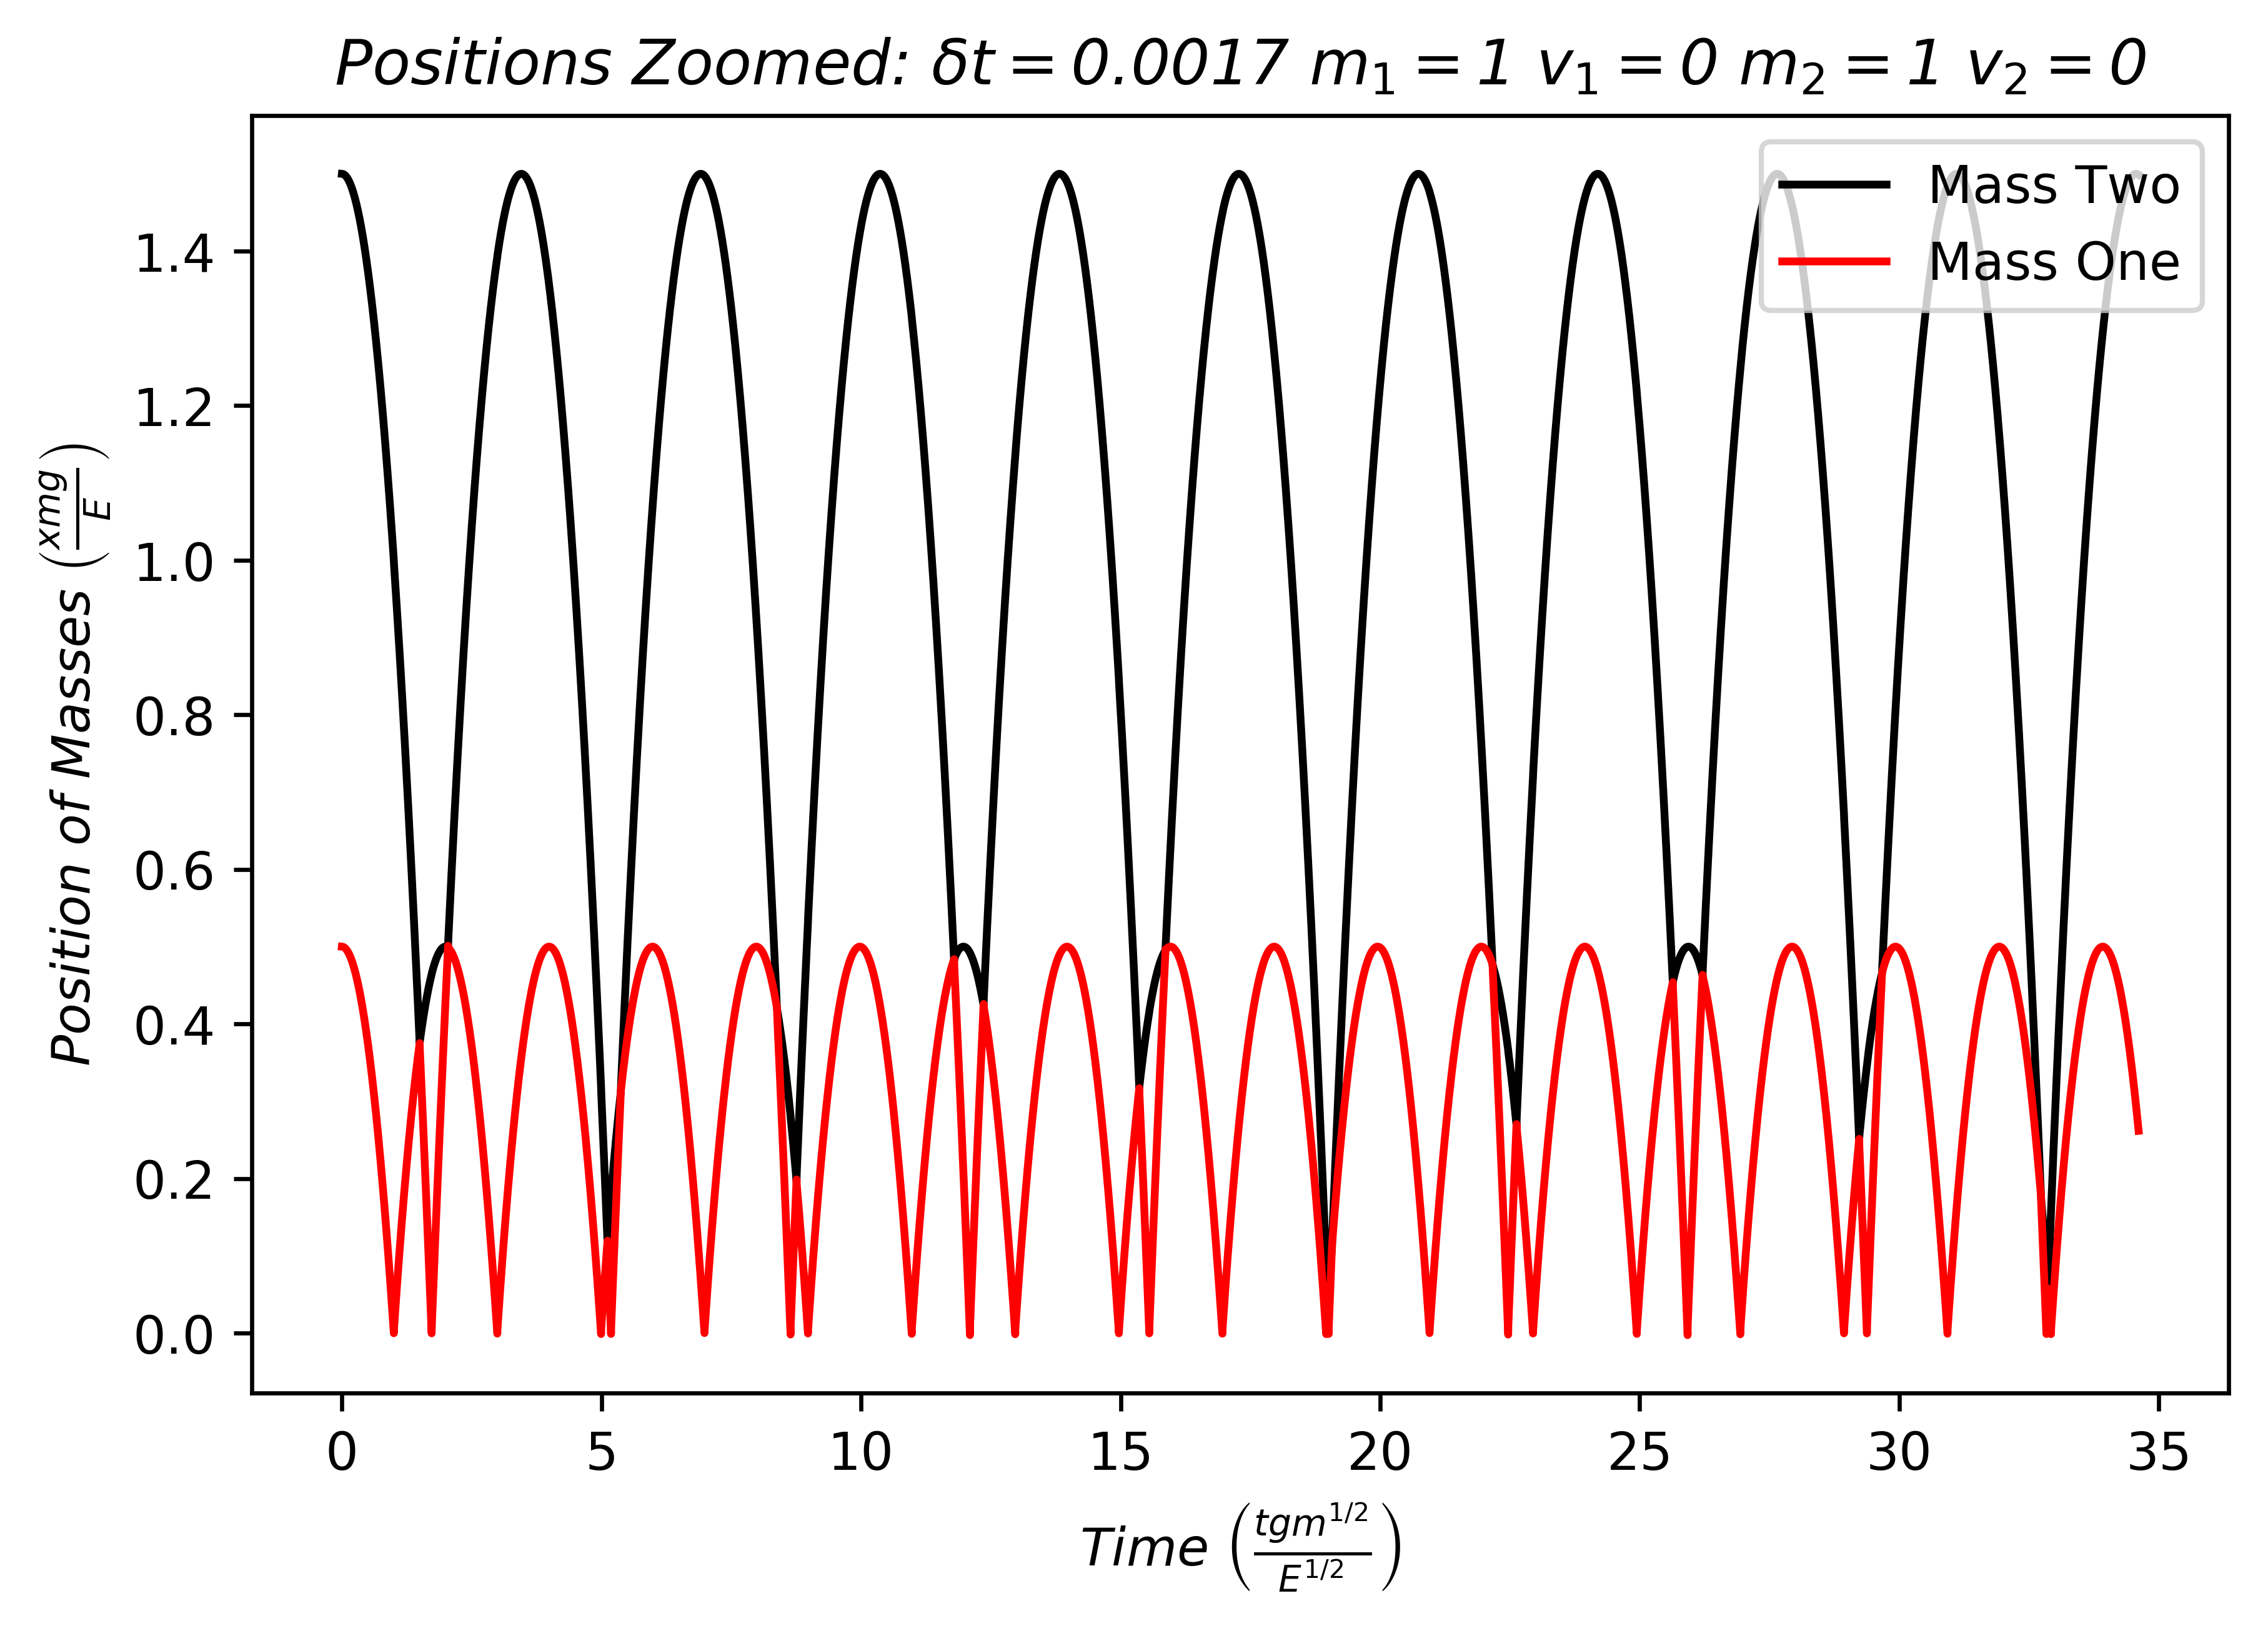
\includegraphics[scale=.45]{PositionsZoomed-MassOne1MassTwo1x1i1x2i3}
\end{figure}
\begin{figure}[h]
\caption{$m_1=1$, $m_2=9$, $x_1=1$, $x_2=3$, $v_1=0$, $v_2=0$}
\centering
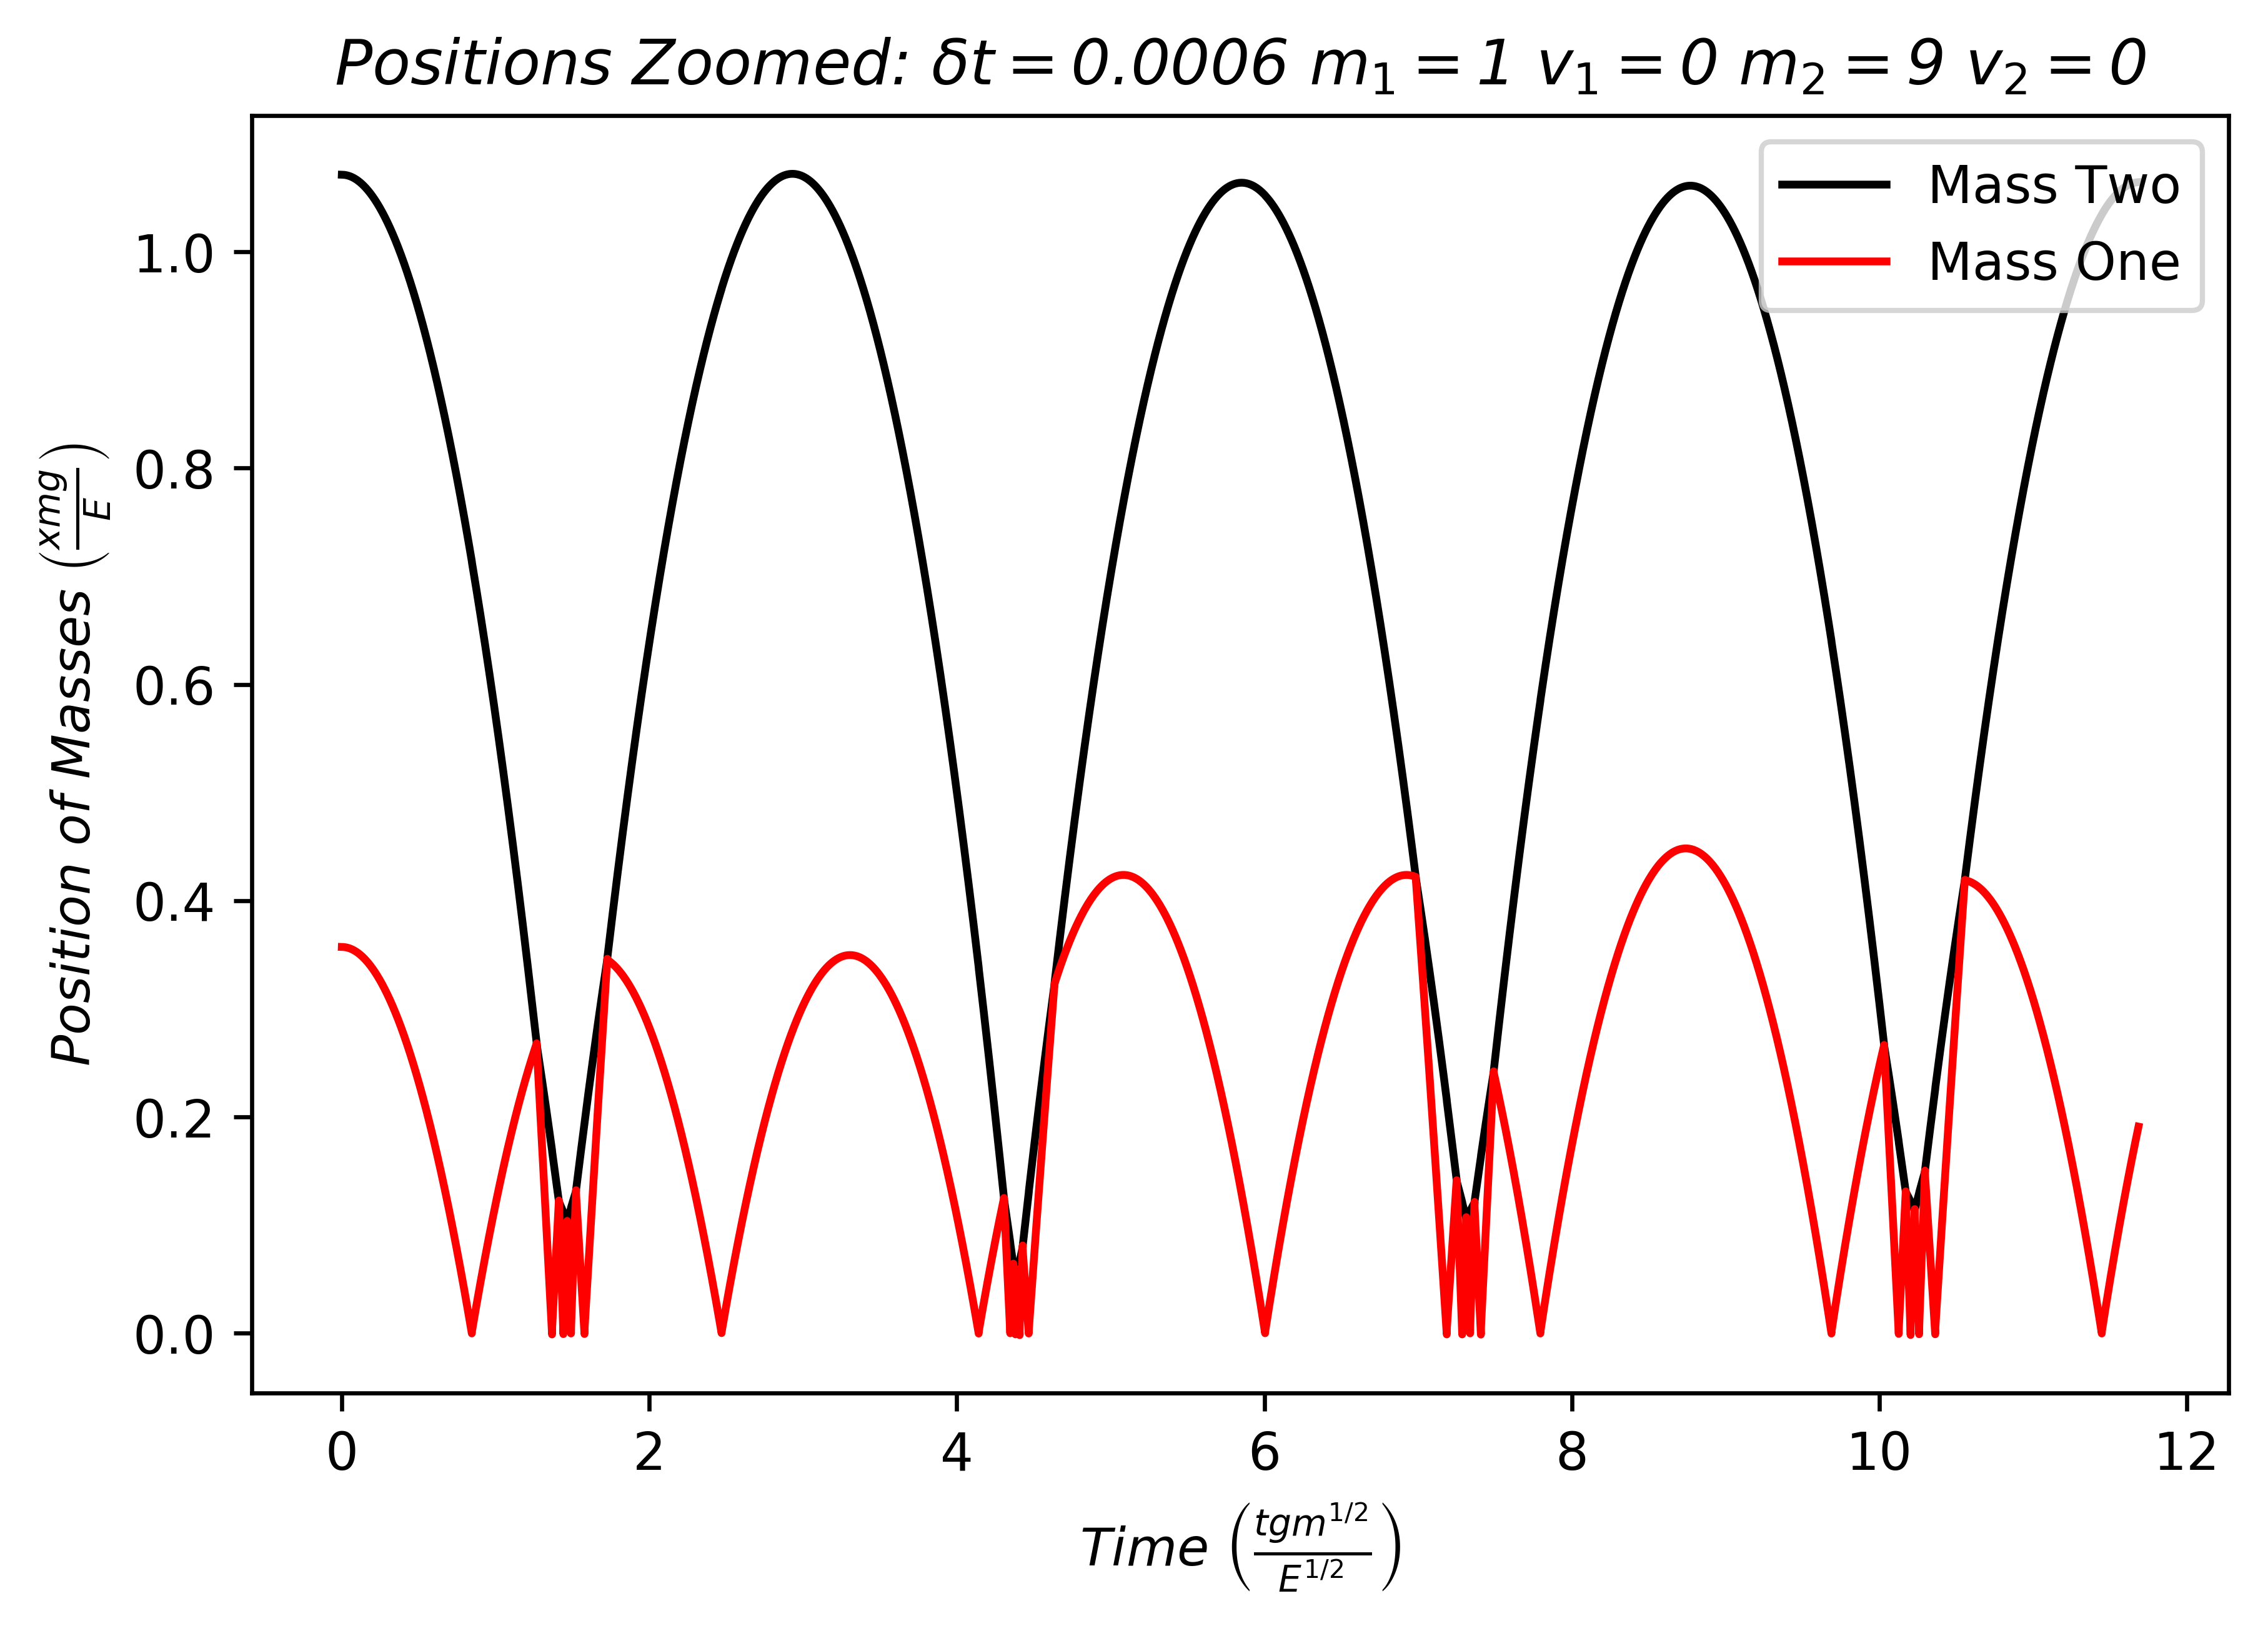
\includegraphics[scale=.45]{PositionsZoomed-MassOne1MassTwo9x1i1x2i3}
\end{figure}
\hspace{-3.8mm}The first set's trajectories (Figure 8) are as random as we expected even within such a short time frame, with only a single short period between $t=20$ and $t=35$  appearing to have any similarity. The second set's trajectories (Figure 9), as expected, also have a very clear periodic pattern that they are following. The third set's trajectories (Figure 10) are a bit odd however, as ball one's behavior appears to be fairly disordered, where as ball two's motion appears quite periodic - at least during this period of time. Regardless of the periodic structures though, the integrity of the simulation does appear to hold over time as the collisions seem to act appropriately.
\subsection{Auto-Correlations}
\hspace{\parindent}Up until now we've merely commented upon the disorder of our plots as a means of measuring the overall chaos of the system. Using an Auto-Correlation Function on the positions of the balls however, gives us the power to quantitatively comment on the level of chaos by calculating the self-similarity the position signal has with itself over time. This means that we should expect the auto-correlation functions of "normal" motions to be constant or oscillating as there should exist patterns over time, where as for chaotic motions we should expect the auto-correlation function to exponentially decay to zero as there should be little self-similarity over time. We can interpret why this is by inspecting the mathematical formula of the auto-correlation function:
\begin{align}
	C(\tau)=\int_{0}^{\infty}[x(t)-\bar{x}][x(t+\tau)-\bar{x}]dt
\end{align}
Here we see that the current position's difference between itself and the mean position is compared to all other positions' difference with the mean position. In other words this indicates that for functions with periodicity, the average difference between a point and the mean should be $0$ or oscillatory over time. In the case of chaotic motion, no pattern should exist over time, hence the auto-correlation function should reduce to zero exponentially. Auto-Correlating the position functions of our three set of initial conditions then, we find that... \\
\begin{figure}[H]
\caption{$m_1=1$, $m_2=0.5$, $x_1=1$, $x_2=3$, $v_1=0$, $v_2=0$}
\centering
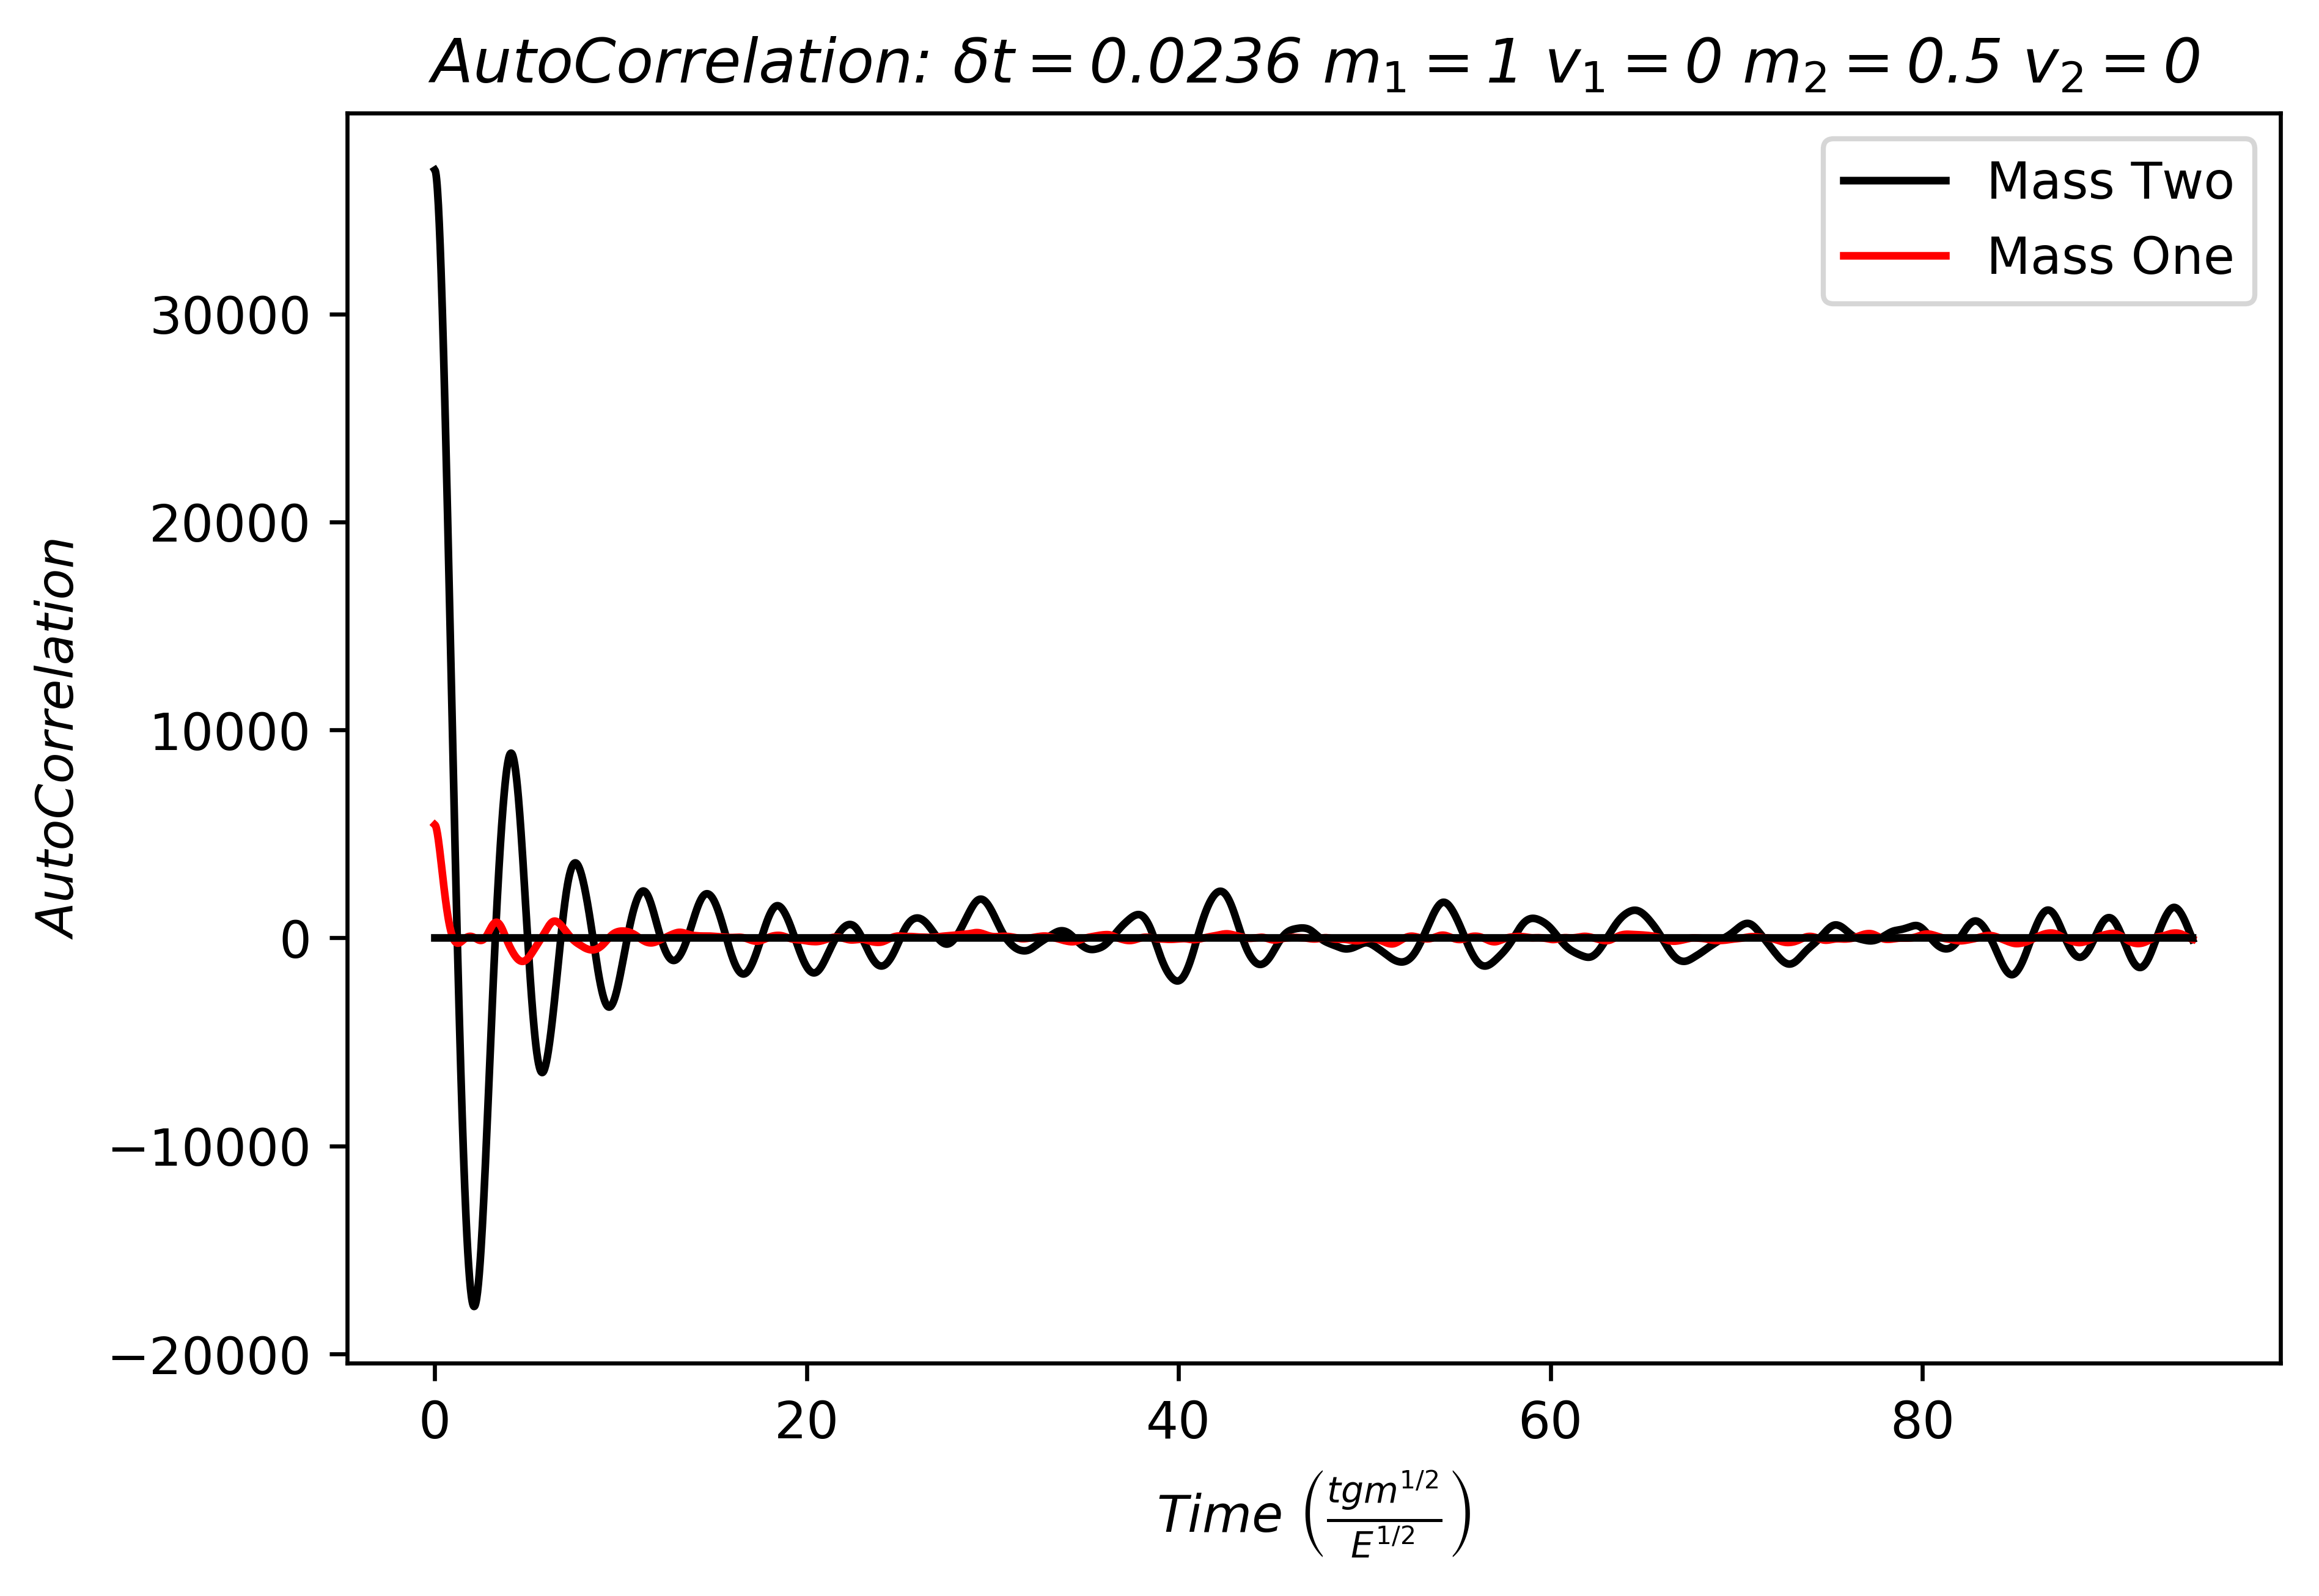
\includegraphics[scale=.45]{Correlation-1-v2}
\end{figure}
\hspace{-3.8mm}Set one (Figure 11) has extremely fast decays for both ball and ball two, indicating that our thoughts on this system being chaotic are correct. We should consider that ball two never decays all the way to zero though, unlike ball one which suggests that there does exist some structural similarities within the positions of ball two over time. That said, there is still no clear oscillation with-in ball two's motion so it is certainly not undergoing "normal" motion. \\
\begin{figure}[H]
\caption{$m_1=1$, $m_2=1$, $x_1=1$, $x_2=3$, $v_1=0$, $v_2=0$}
\centering
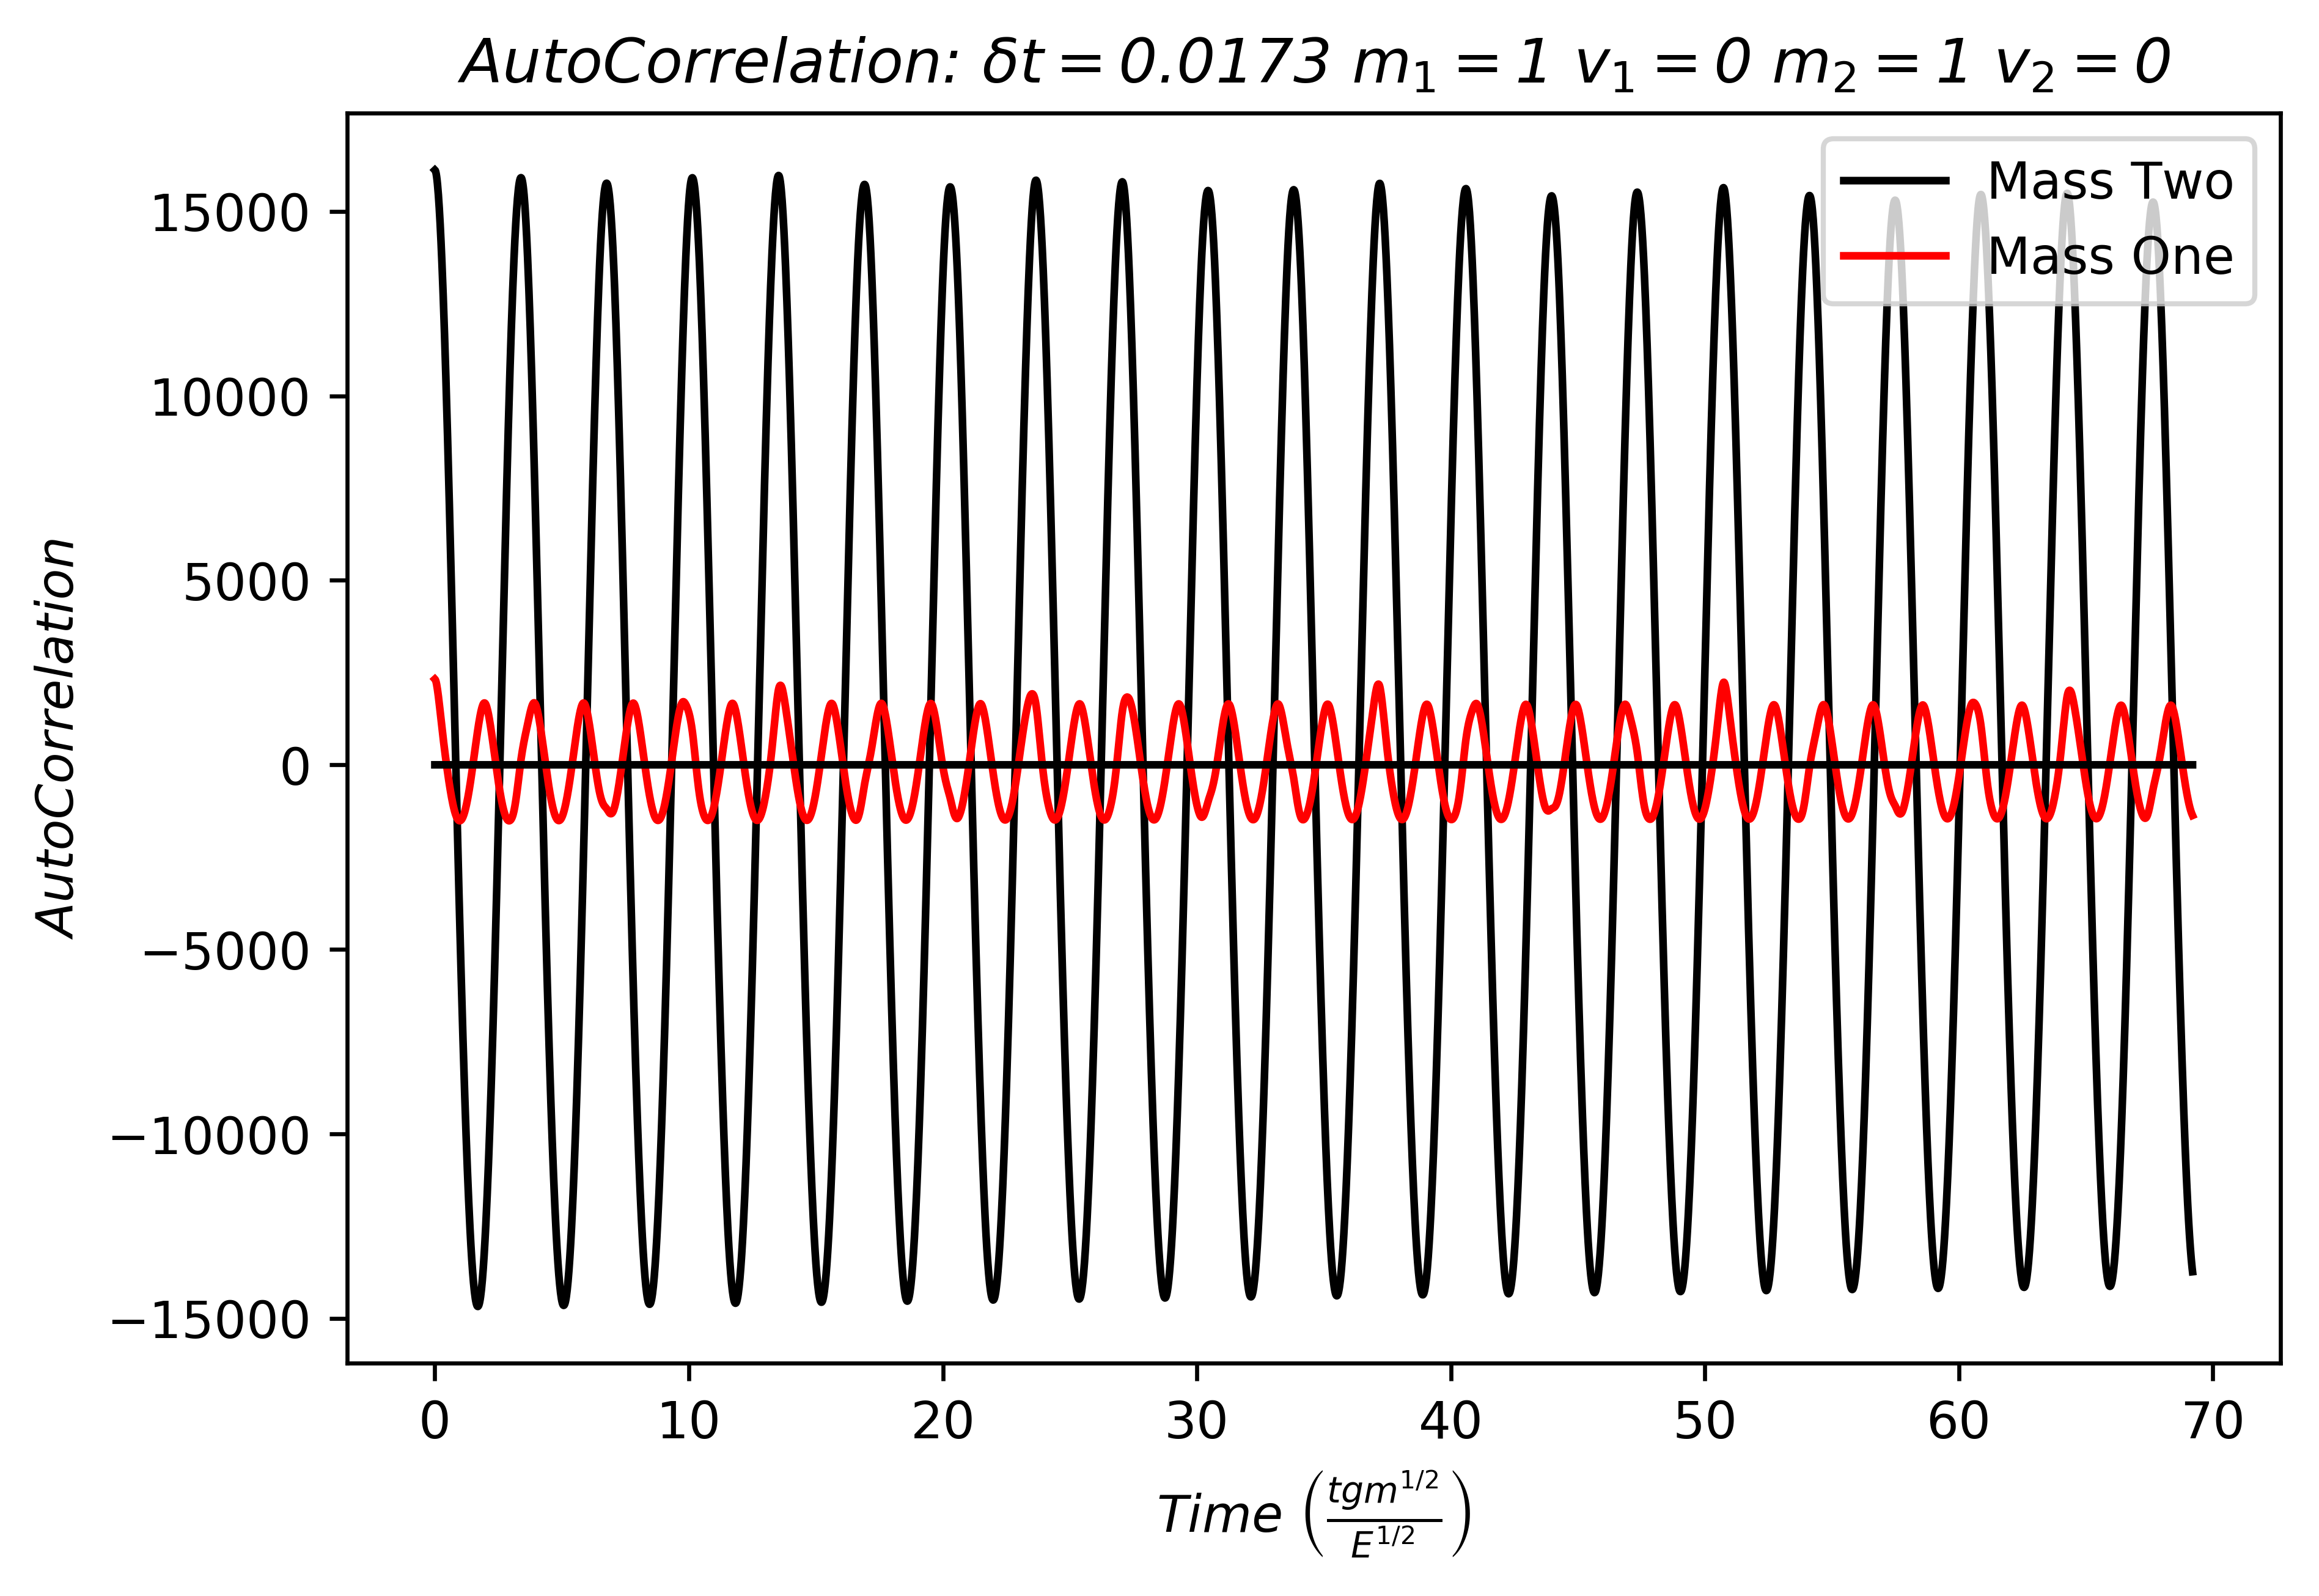
\includegraphics[scale=.45]{Correlation-2-v2}
\end{figure}
\hspace{-3.8mm}Set two (Figure 12) clearly has a very distinct oscillatory pattern for each of its balls' auto-correlation functions, which is exactly what we should expect of our most ordered system. It is interesting to note that ball two's auto-correlation has a much larger amplitude than ball one's but this is simply because of ball two's much larger range of motion compared to ball one's. \\
\begin{figure}[H]
\caption{$m_1=1$, $m_2=9$, $x_1=1$, $x_2=3$, $v_1=0$, $v_2=0$}
\centering
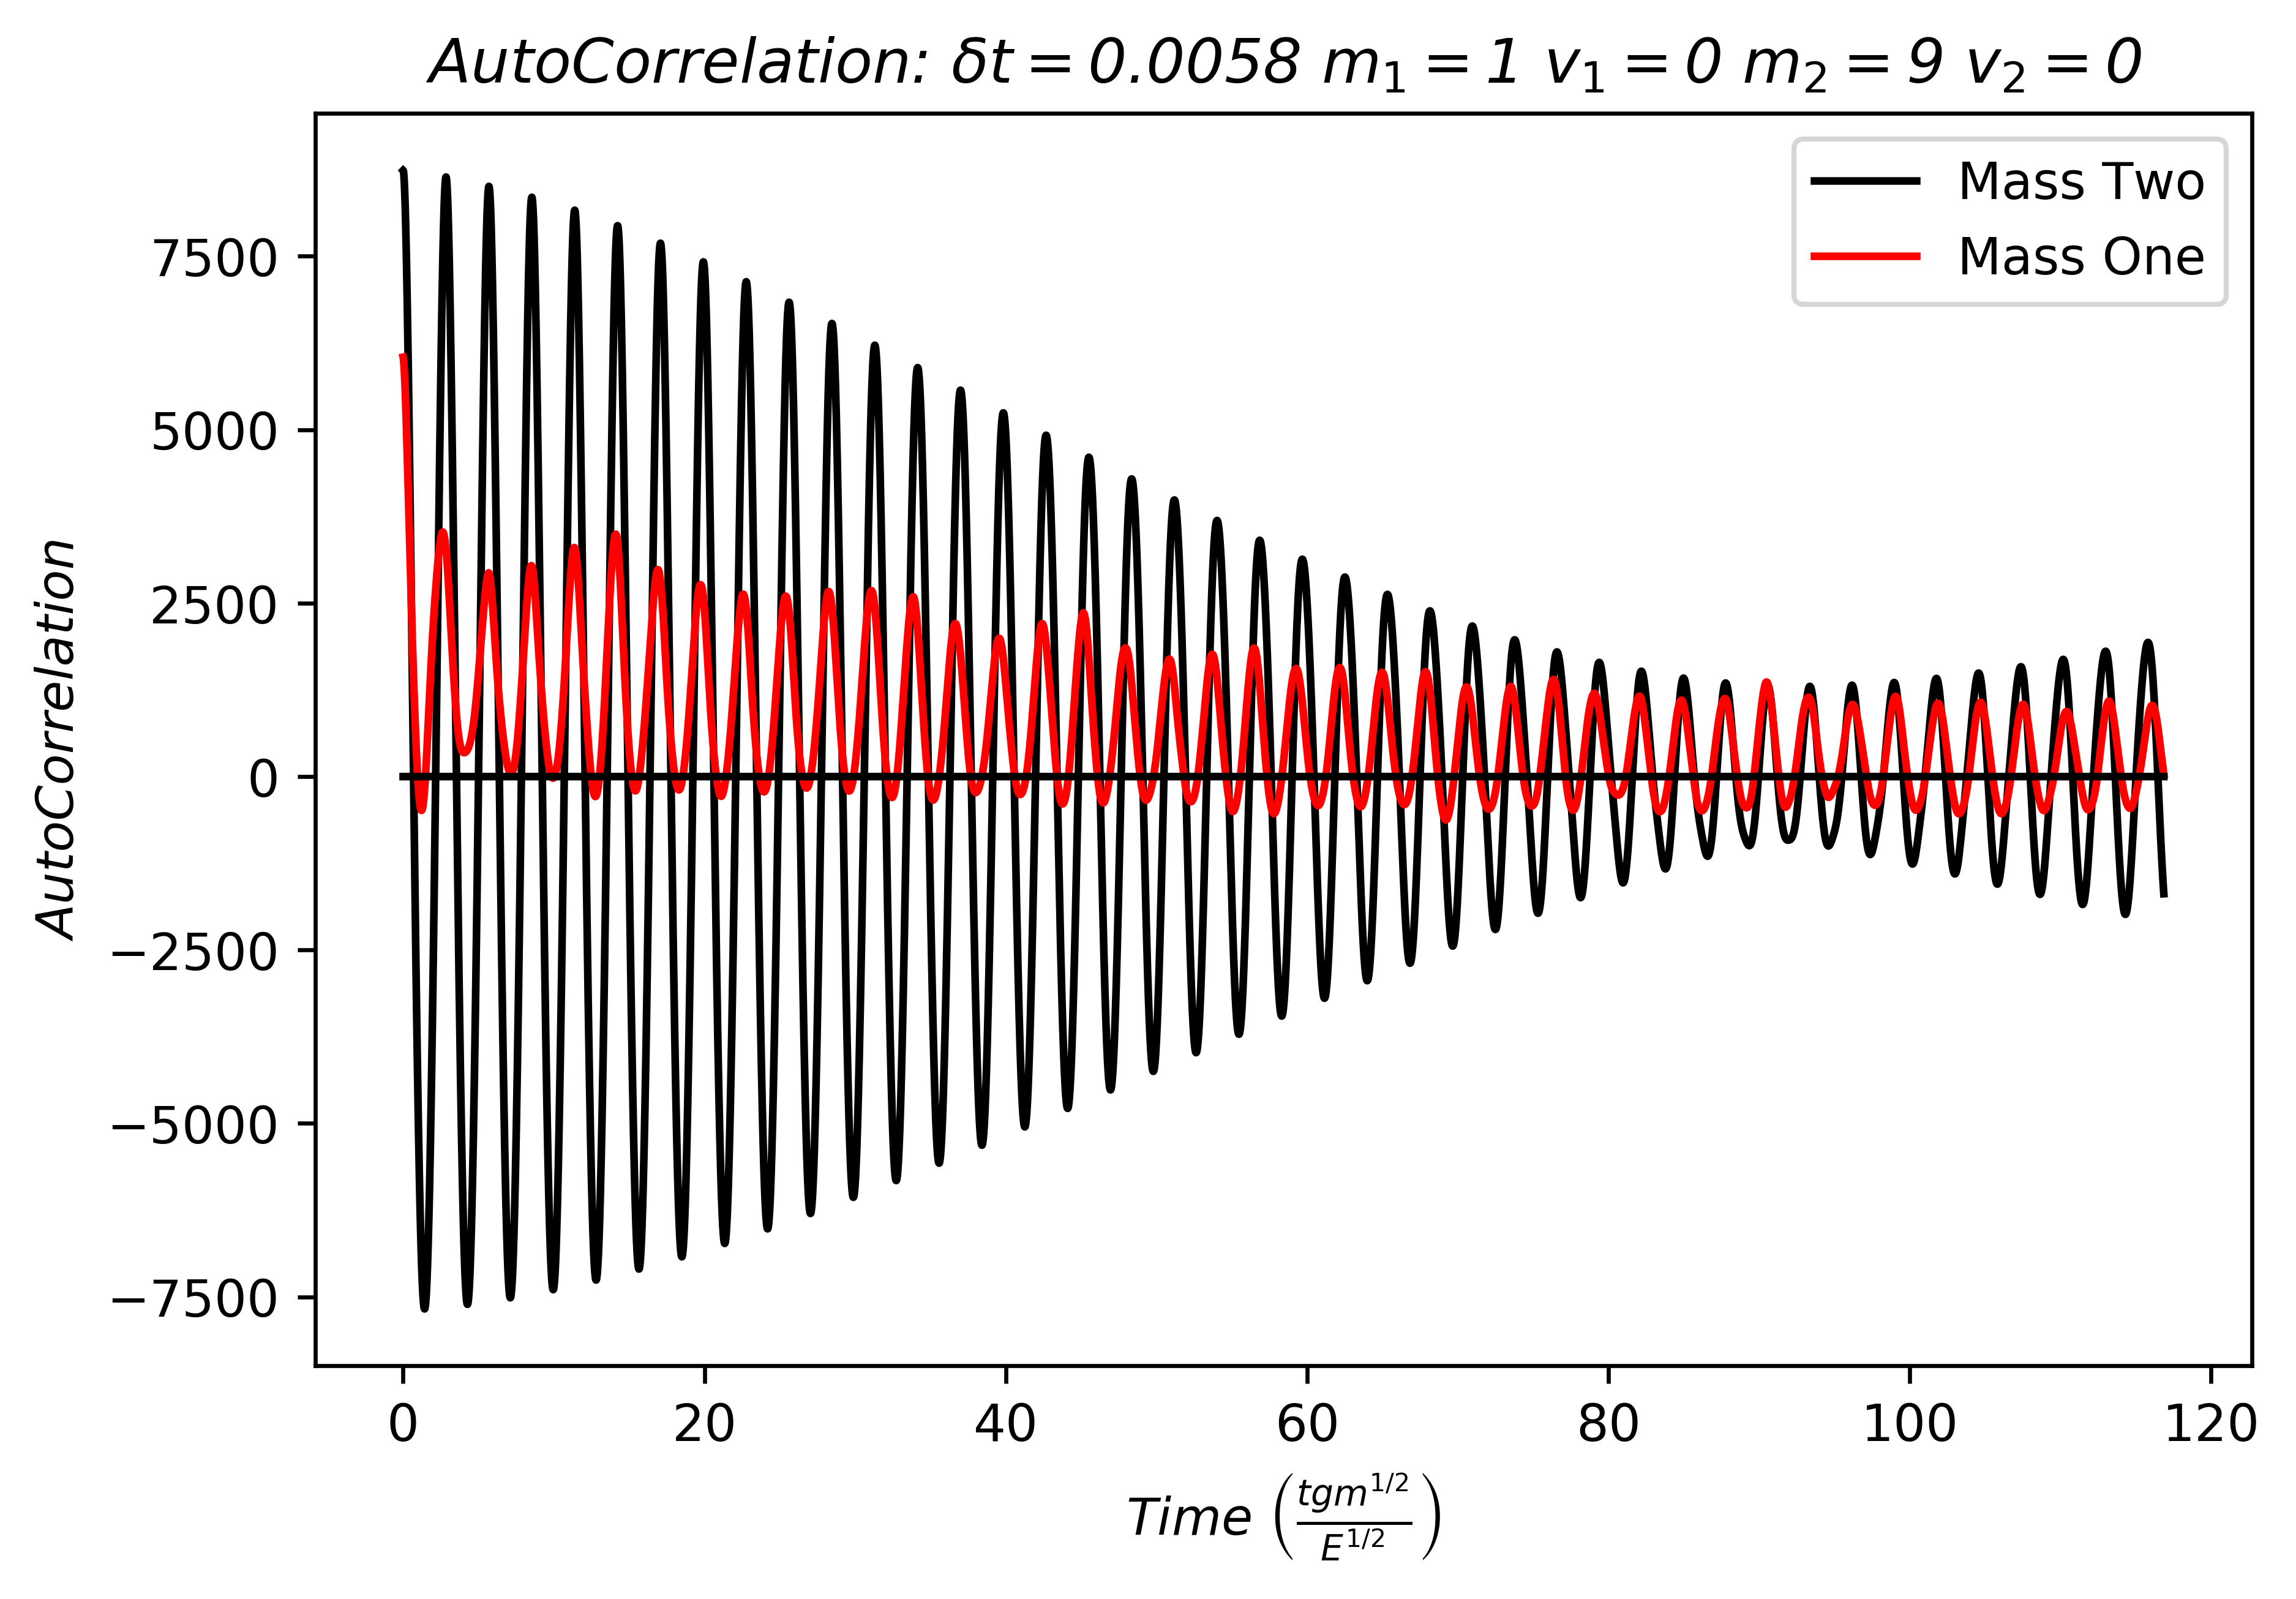
\includegraphics[scale=.45]{Correlation-3-6}
\end{figure}
\hspace{-3.8mm}Set three (Figure 13), similarly to set one, experiences an exponential decay on both balls, but unlike set ones' its decays is much more gradual and only tends towards zero rather than reaching it. This is probably a consequence of the number of collisions recorded. Given more collisions the topology of the system would have more time to evolve which would in turn cause the auto-correlation of the two balls' positions to decay towards zero much more dramatically. Nevertheless, the exponential decay is a clear indicator that the system with set three's initial conditions is chaotic. 

As a final examination of the auto-correlation function, lets alter the initial conditions of set three such that the new system's Poincar'e section becomes more orderly - as in Figure 2 - and then inspect the differences between the two respective auto-correlation plots. By following the method as outlined in \textit{Two Balls in One Dimension with Gravity}$^{[4]}$, we can find that this altered set of initial conditions is approximately $x_1\approx0$, $x_2\approx.75$. Hence, we find that our new Poincar'e section and accompanying auto-correlation plot are:
\begin{figure}[H]
\caption{$m_1=1$, $m_2=9$, $x_1=0.01$, $x_2=0.75$, $v_1=0$, $v_2=0$}
\centering
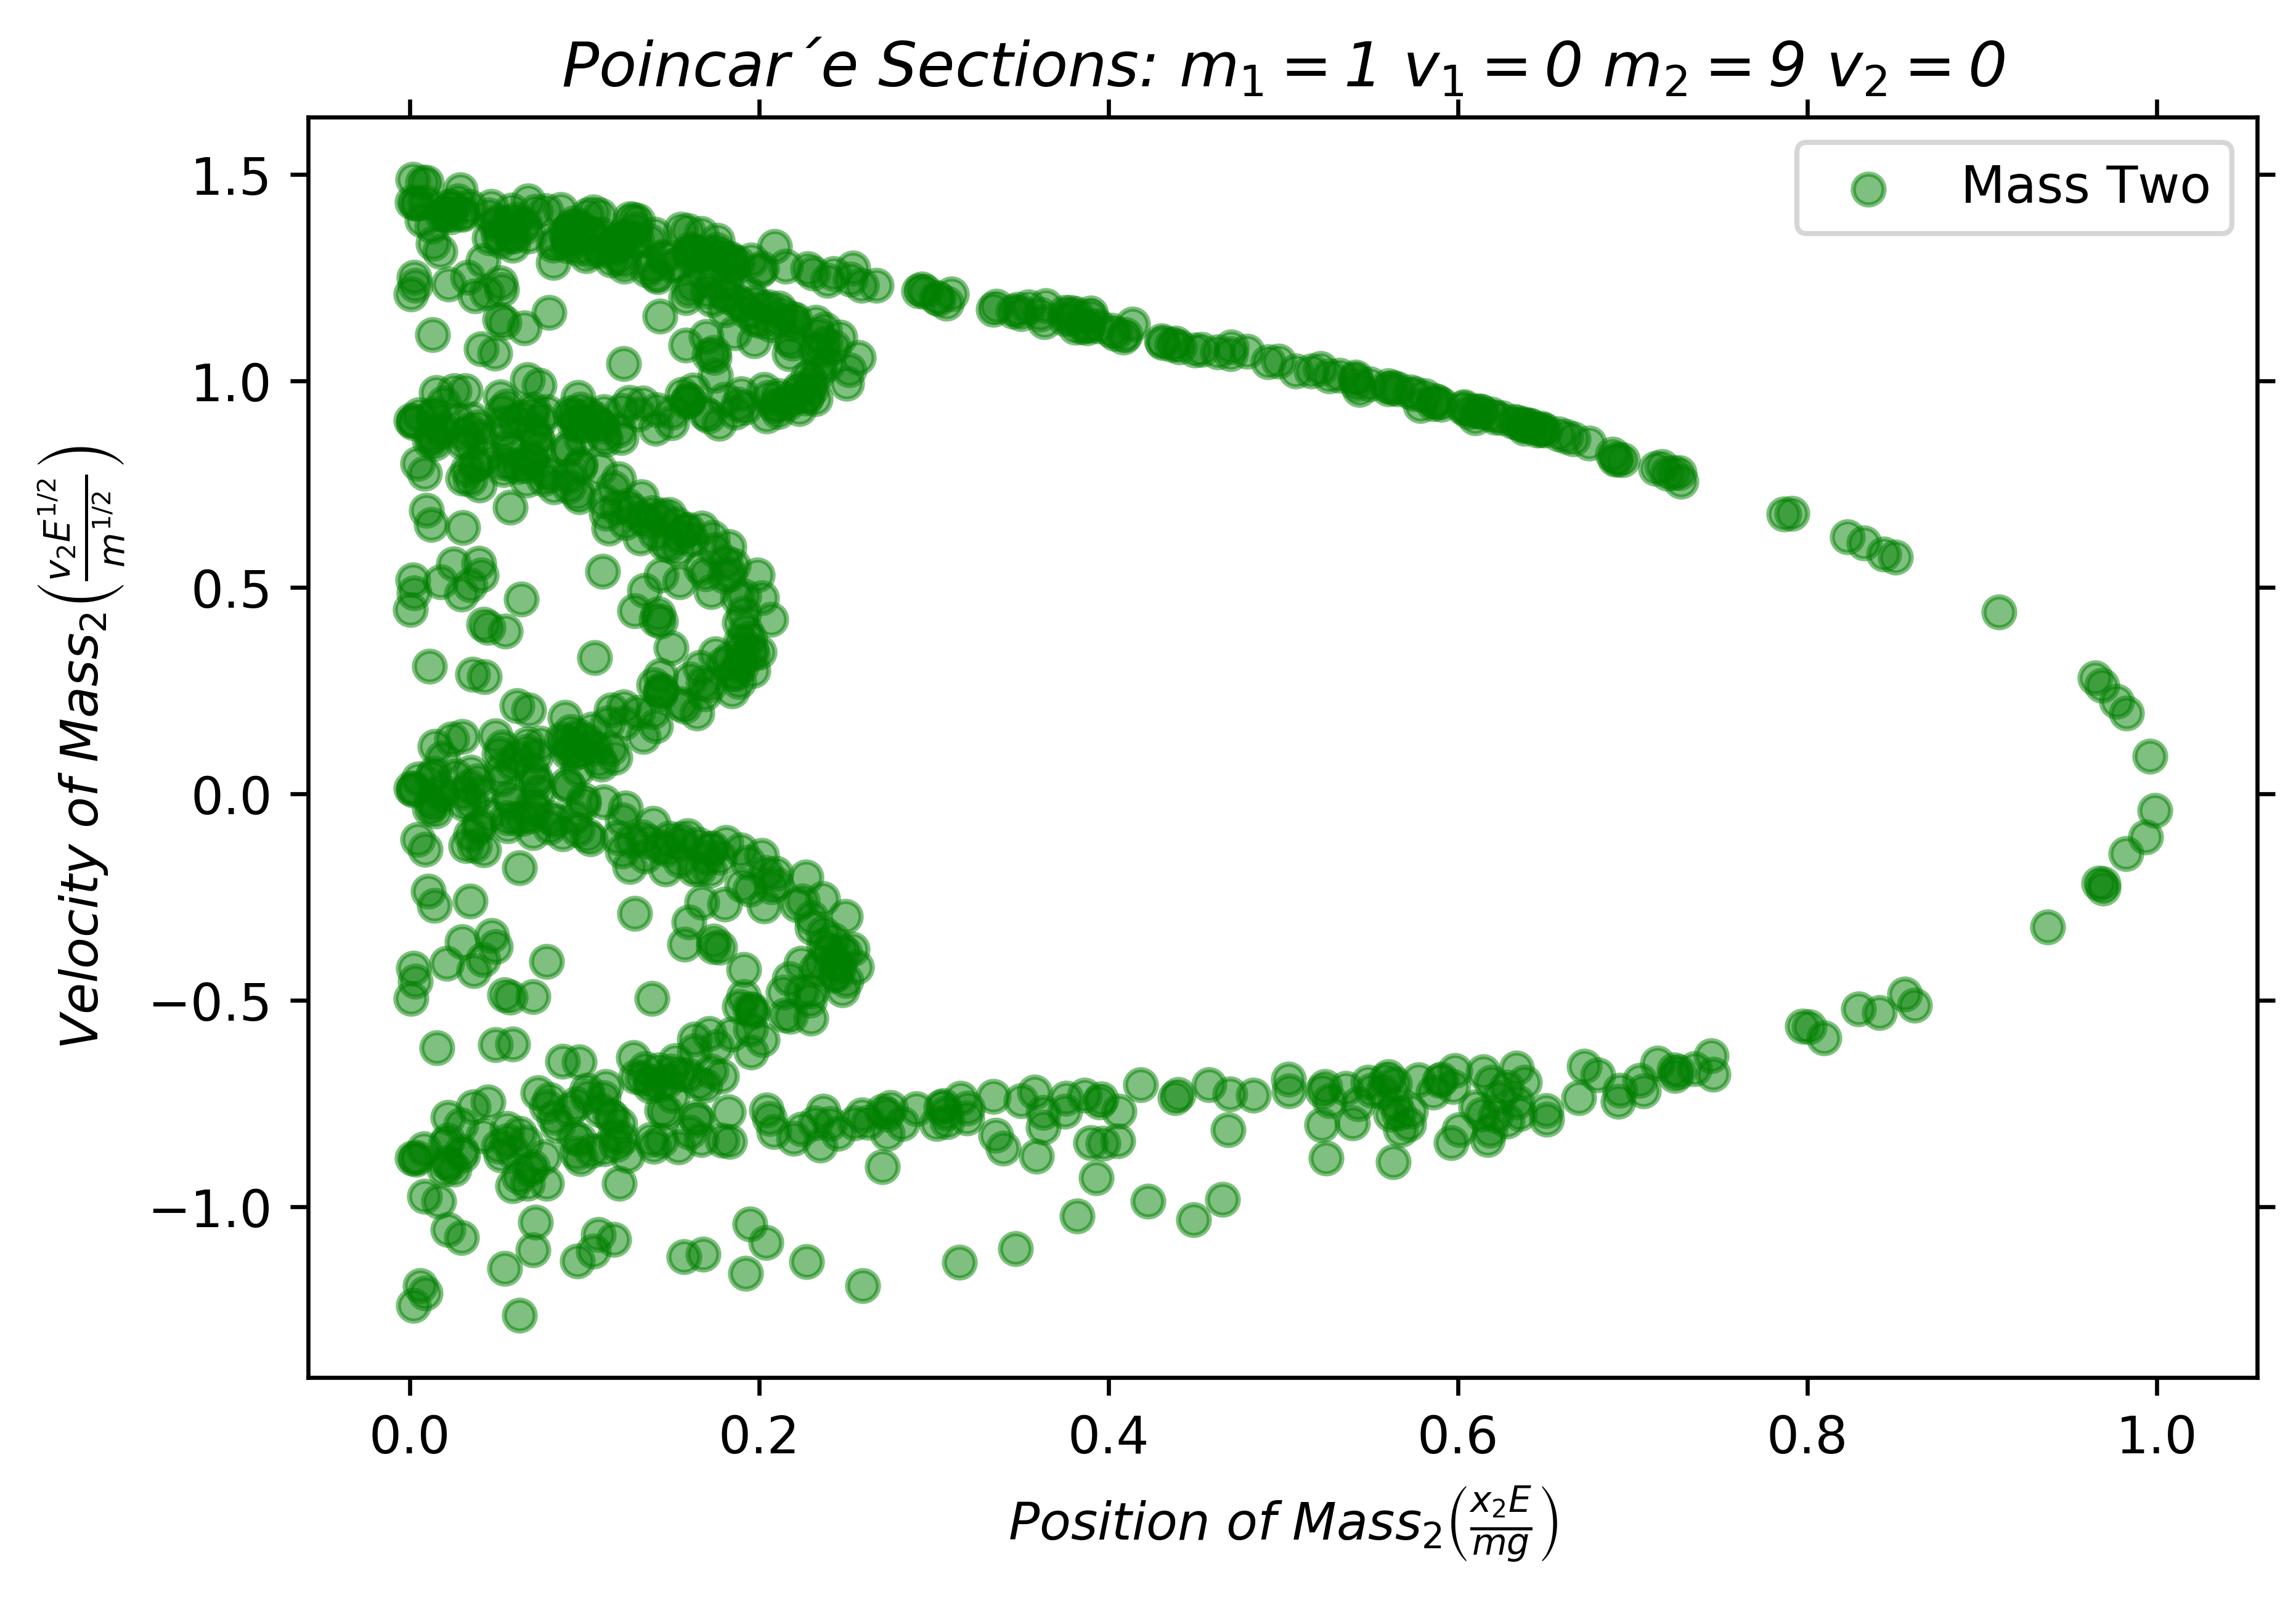
\includegraphics[scale=.45]{Section-MoreNormal}
\caption{$m_1=1$, $m_2=9$, $x_1=0.01$, $x_2=0.75$, $v_1=0$, $v_2=0$}
\centering
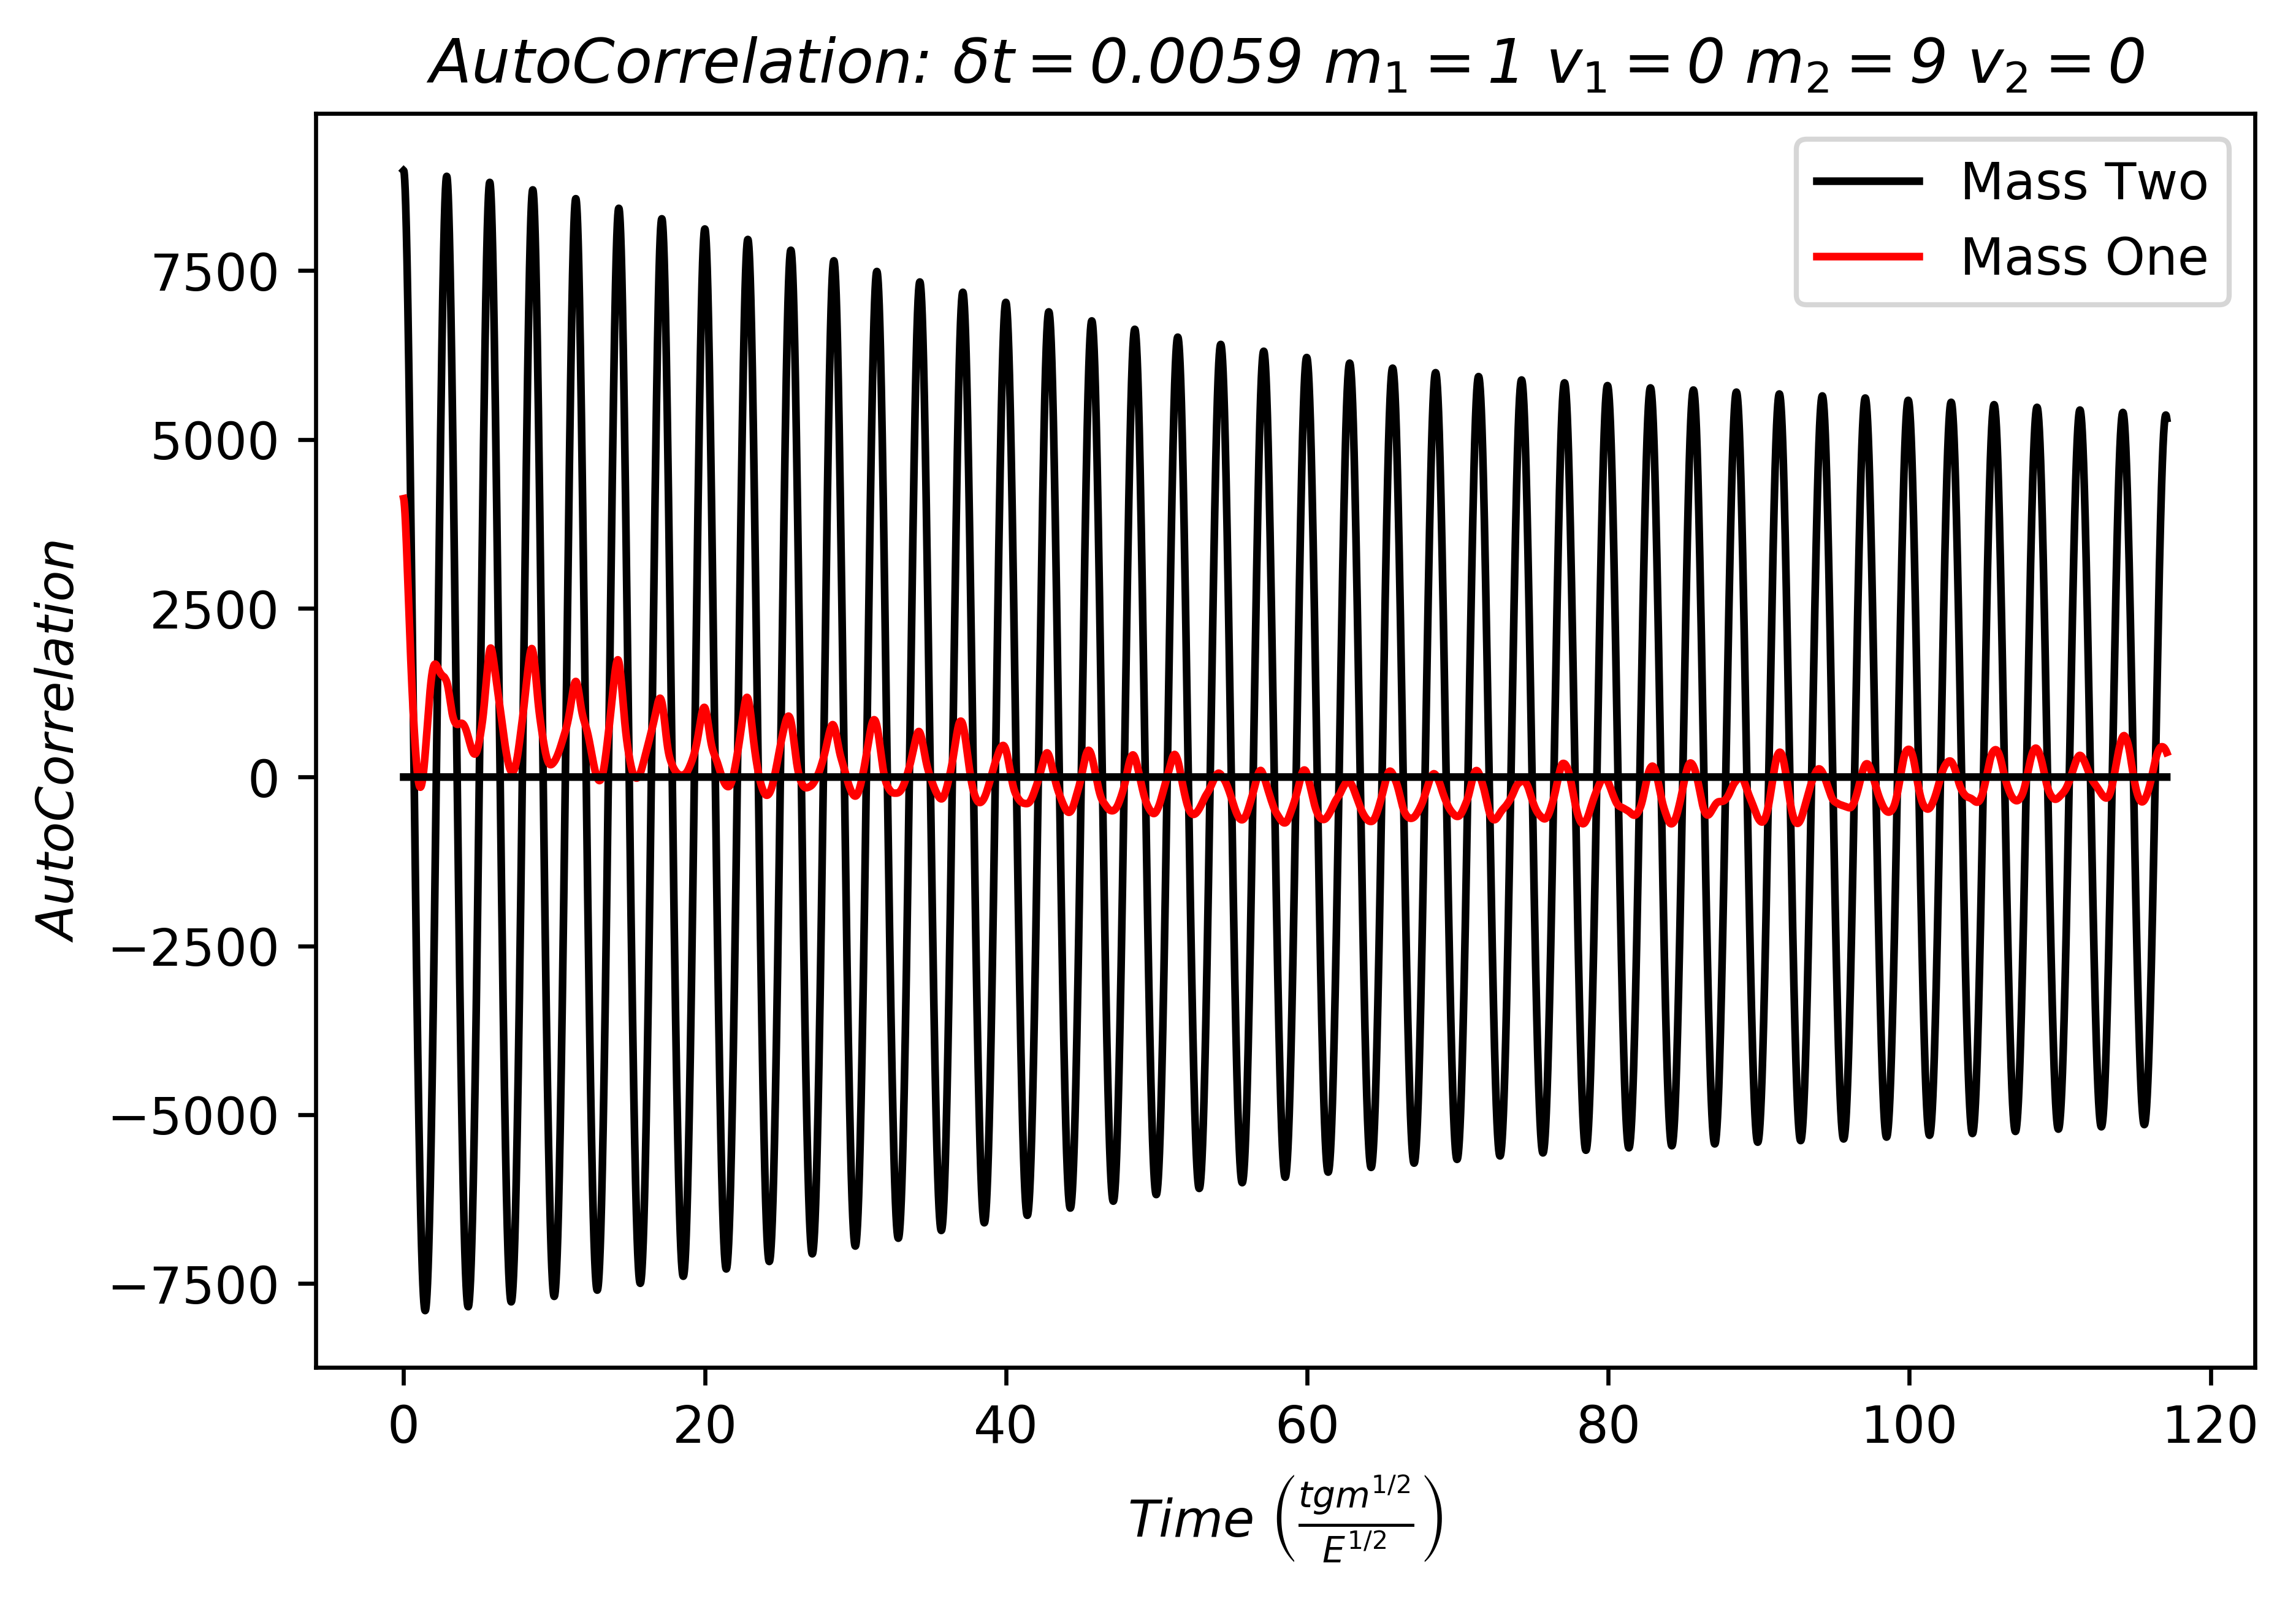
\includegraphics[scale=.45]{Correlation-MoreNormal}
\end{figure}
Figure 14 has a very distinct line akin to Figure 2 which indicates that our altered initial conditions really are more ordered. This becomes even more abundantly clear when we look at the corresponding auto-correlation function (Figure 15). There is certainly still decay within both ball's functions; however, the decay is certainly much less than in the case of the original set of initial conditions. This indicates that by changing the initial conditions of a chaotic system it is possible to make its motion significantly more ordered to the point that its motion is "normal" or in our case approximately "normal". 
\subsection{Lyapunov Exponent}
\hspace{\parindent}The Lyapunov exponent is a measurement of the rate of separation between two trajectories that start infinitesimally close to one another. This is a convenient tool for us, because it allows us to mathematically measure just how sensitive our system is to changes in its initial conditions. This calculation works by taking two points in space with an initial separation $\delta{Z}(0)$, and measuring how much they diverge from one another over time in the form:
\begin{align}
	\left|\delta Z(t)\right| \approx \left|\delta Z(0)\right| e^{\lambda t}
\end{align}
where $\delta Z(t)$ is the magnitude of the difference between the two motions over time and $\lambda$ is the Lyapunov exponent. This means that the larger the Lyapunov exponent, the quicker the two trajectories diverge one another. Given this tool then, lets see how the Lyapunov exponent of the chaotic case of set three compares to the "normal" case of modified set three seen in Figure 21. We should expect that the chaotic case will have a greater Lyapunov exponent than the "normal" case because of the topological mixing and sensitivity to initial conditions present in chaotic systems. These properties of course should cause drastic changes in the positions being measured that wouldn't be as prevalent in the "normal" case, hence, resulting in a larger exponent. For our test, we will calculate their respective Lyapunov exponent by comparing their initial conditions against an identical set of initial conditions that has an $x_2$ value that is $10^{-6}$ greater than the original. Running our simulations we find that: \\
\begin{figure}[H]
\caption{$m_1=1$, $m_2=9$, $x_1=1$, $x_2=3$, $v_1=0$, $v_2=0$}
\centering
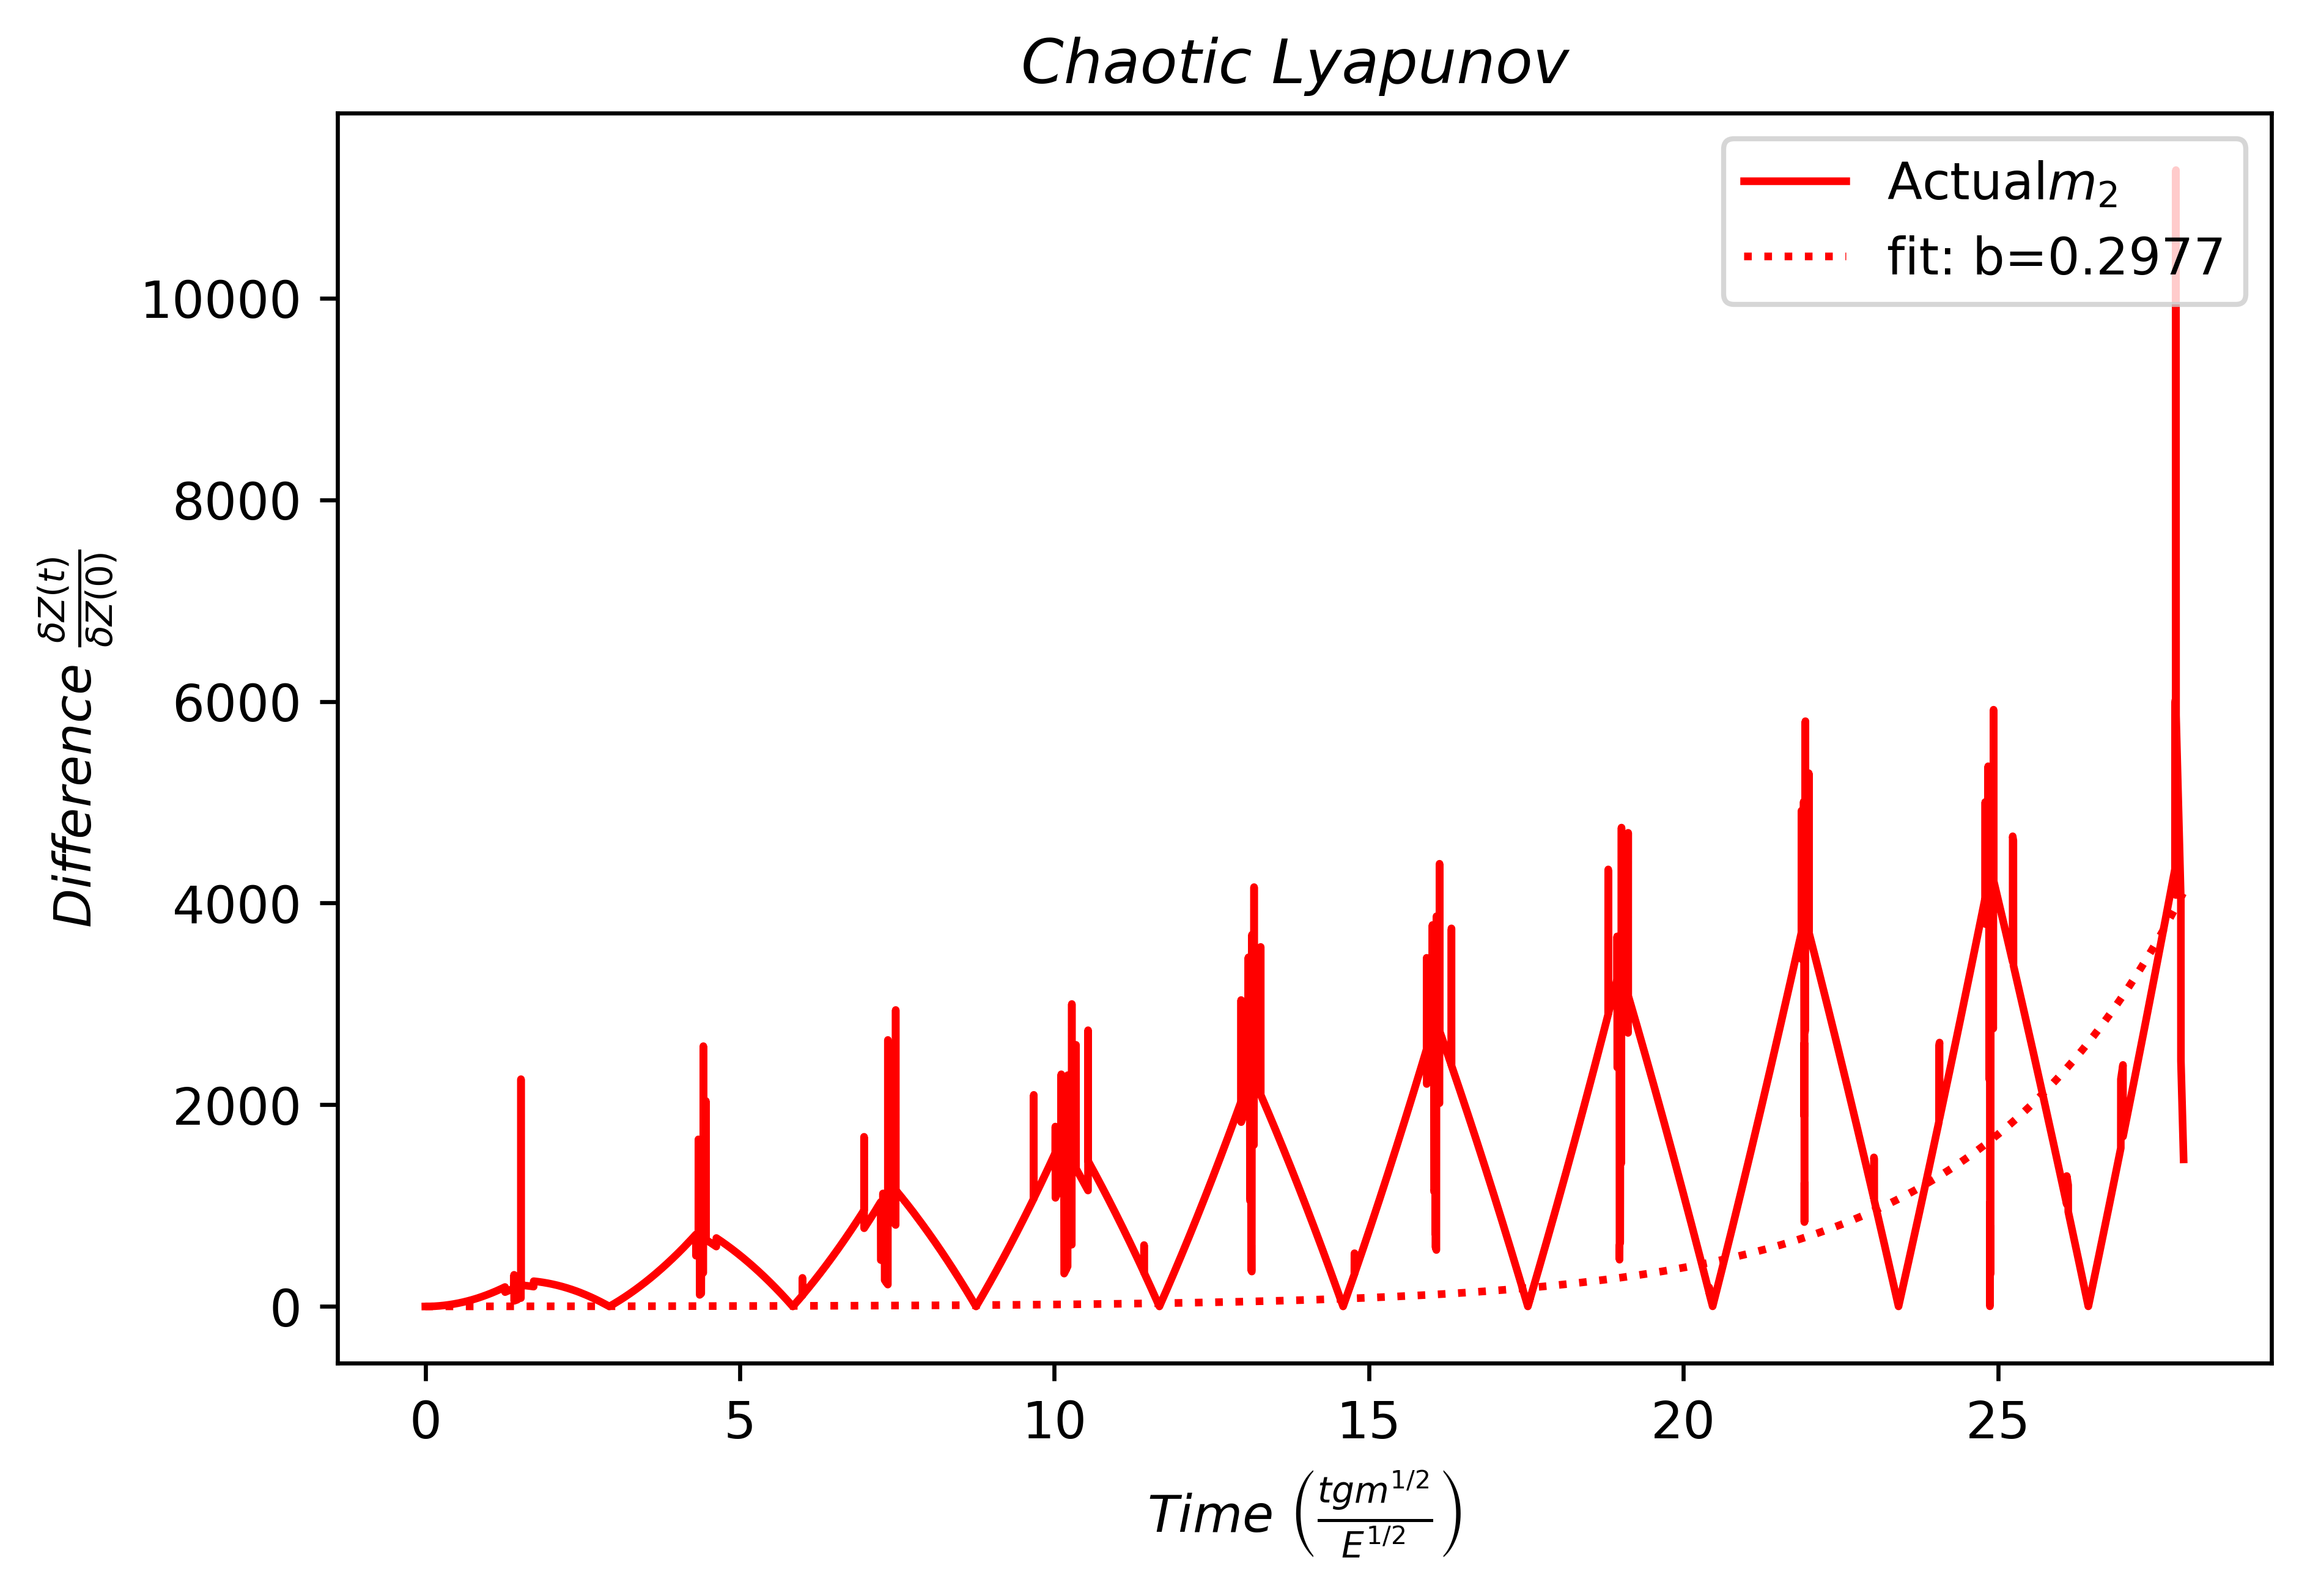
\includegraphics[scale=.45]{ChaoticLyapunov1}
\end{figure}
\begin{figure}[H]
\caption{$m_1=1$, $m_2=9$, $x_1=1.4$, $x_2=2.6$, $v_1=0$, $v_2=0$}
\centering
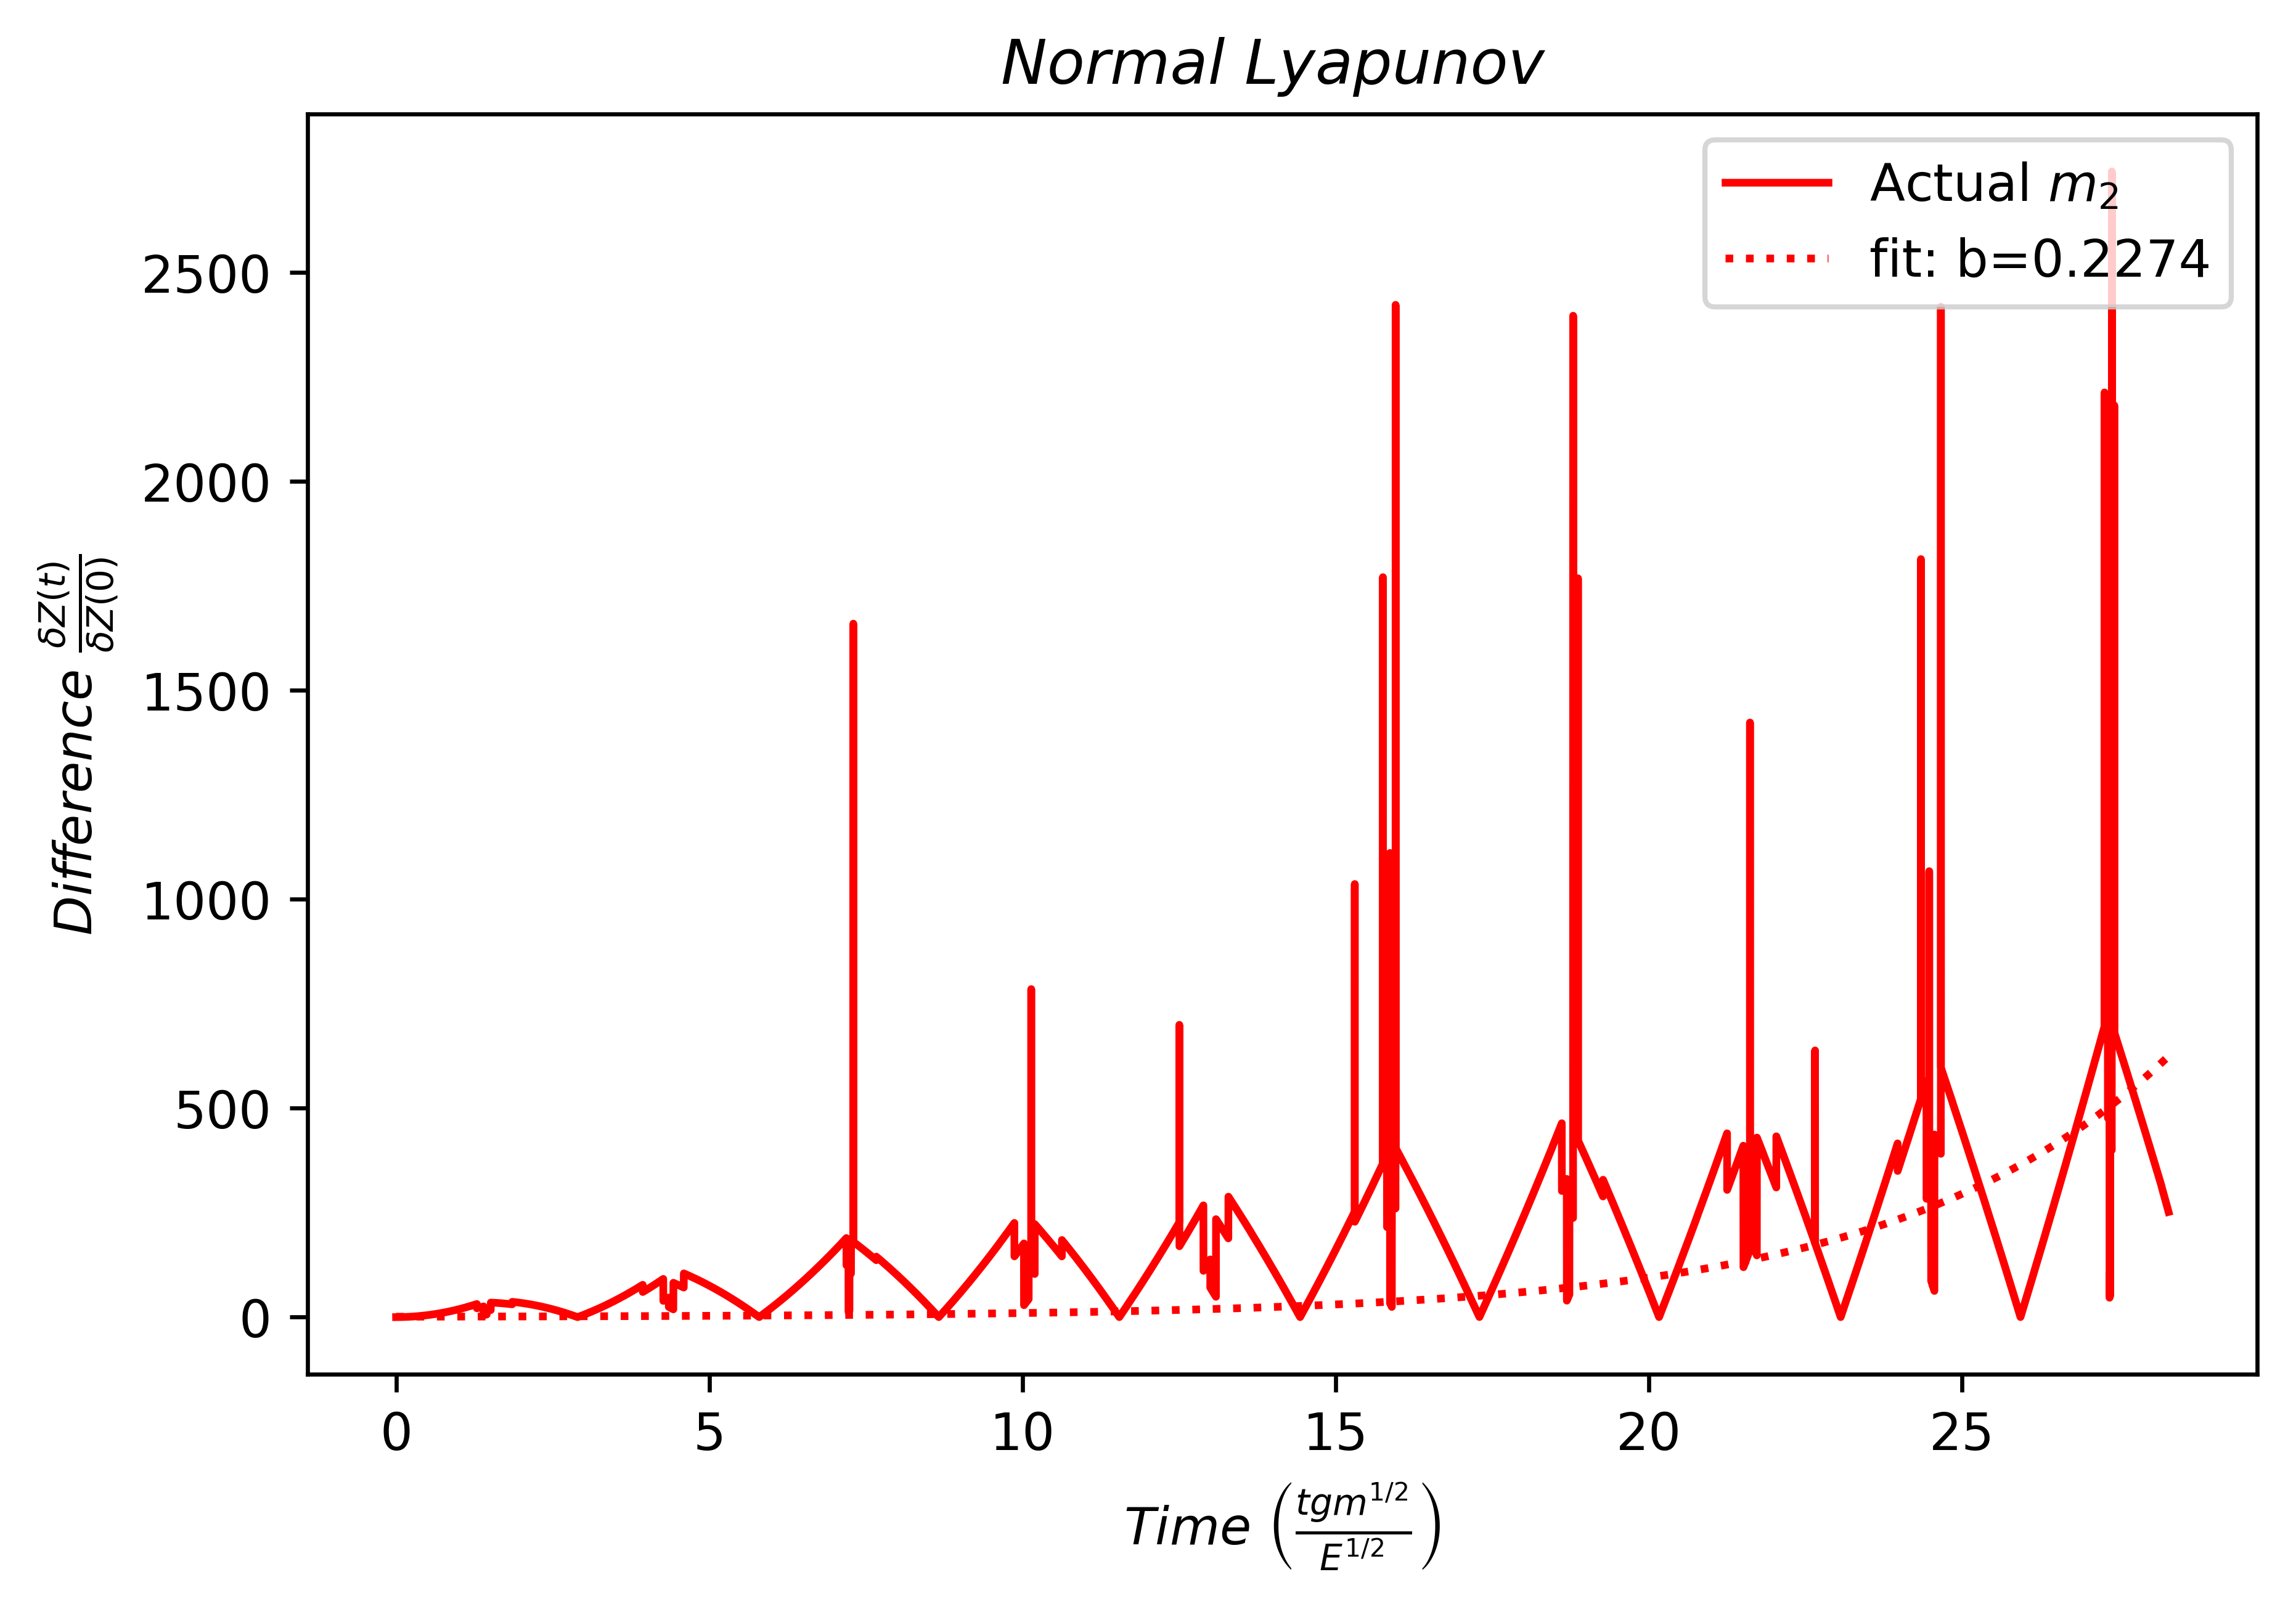
\includegraphics[scale=.45]{NormalLyapunov1}
\end{figure}
\hspace{-3.8mm}where the fit quantity $\lambda$ refers to the value of the Lyapunov exponent. As we expected the Lyapunov exponent for our chaotic system is certainly larger than the "normal" one.
\section{Conclusion}
\hspace{\parindent}From our simulations, we have found that there are many analytical models we can use to help us interpret chaotic systems. For our particular system, we used two balls constrained to an axis that lied parallel to the gravitational pull of Earth such that there existed only two degrees of freedom. The reason for using so few degrees of freedom was to limit the complexity of the system, so that interpretations would be easier to make and consequentially fundamental intuitions about chaotic systems in general would come more naturally. Using Poincar'e sections we were able to gain our first ideas about chaotic systems by observing the topological structures and substructures of our three sets of initial conditions. From these plots we determined that our first set of initial conditions was the most chaotic because of its near complete lack of structure. By the same logic we also came to the conclusion that the second set was the most ordered because of how clean and distinct its two structures were. Unlike the first set, we found that the third set certainly had distinct structures, but that unlike the second set they were not as "clean" cut. Once, we got accustomed to interpreting these plots, we decided to observe how small changes to the initial conditions of set two could change its Poincar'e section. We did this by overlaying twelve of these modified set twos over top of one another and found that small changes to the initial conditions of set two were able to cause massive changes in their respective Poincar'e sections. After interpreting the topological features of the Poincar'e plots, we explored the position plots of our same three sets of initial conditions. As we expected from our observations of their respective Poincar'e sections, the first set was again the most chaotic - especially when we zoomed in to see exactly how the balls interacted with one another. The second set also exactly as expected, maintaining a very precise periodicity. The third set however, was slightly unexpected. We had originally predicted that its position plot would have a similar number of structures as its Poincar'e section but this was not the case, particularly over all time. Despite this, our prediction was not entirely wrong as there still existed periods of distinct structures.

Once we had finally established a good idea as to the state of the systems arising from the different sets of initial conditions, we decided to determine the absolute truth mathematically through the auto-correlation function. The auto-correlation functions measures the self-similarity of a signal, which of course makes it perfect for determining how chaotic a system is because the more chaotic it is the more quickly the function will decay to zero. Calculating the auto-correlation function of each set we finally proved what we had suspected all along! That the first set of conditions was indeed the most chaotic of them all, the second set the least, and the third set lying somewhere between the two. Similarly to our tests with the Poincar'e sections we also modified the initial conditions of set three to see if we could make the system's motion "normal" or at least close to it. Although we weren't able to accomplish this perfectly, we were able to get pretty close using the modified conditions $x_1=0.01$ and $x_2=0.75$ and proved that the more ordered a system is, the less decay there is present. Finally, we calculated the Lyapunov Exponent of our third set and modified third set as seen in Figure 15, when compared to identical set of initial conditions with an $x_2$ position that was $10^{-6}$ greater than the original. Our prediction that the Lyapunov exponent of the chaotic system would be larger than the "normal" one proved to be correct!. We reasoned that this was because of the topological mixing present in the chaotic system which would lead to more random motion; and hence, greater discrepancies in the distance between the two different $x_2$ positions. 
\begin{thebibliography}{9}
\bibitem{latexcompanion} 
Shivakumar Jolad
\textit{Poincare Map and its application to 'Spinning Magnet' Problem}.
(2005)
\bibitem{latexcompanion} 
Pesin, Y.B
\textit{Characteristic Lyapunov Exponents and Smooth Ergodic Theory}. 
(1997).
\bibitem{latexcompanion} 
Giordano, Nakaishi.
\textit{Computational Physics 2nd Edition}. 
Pearson Education, Inc. (2006).
\bibitem{latexcompanion}
N. D. Whelan,D. A. Goodings, and J. K. Cannizzo
\textit{Two Balls in One Dimension with Gravity}
(1998).
\end{thebibliography}
\end{document}